% FalconVQA — Software Design Document
%
% Main file. Packages and styling live in preamble.tex; each section is its own
% file under sections/. The \input order below, not the filename prefix,
% is what sets section numbering, so to reorder the report, reorder these lines.
% To work on one section alone, comment the others out; numbering and the table
% of contents adjust on their own.

\documentclass[11pt,a4paper]{article}

% Packages, styling and shared macros. Included by report.tex.

\usepackage[margin=1in]{geometry}
\usepackage{amsmath}   % \text in the fusion equation, Section 5
\usepackage{graphicx}
\usepackage{booktabs}
\usepackage{tabularx}
\usepackage{enumitem}
\usepackage{xcolor}
\usepackage{titlesec}
\usepackage[hidelinks]{hyperref}
\usepackage{caption}
\usepackage[section]{placeins}
\usepackage{tikz}
\usetikzlibrary{positioning,arrows.meta}

% Keep every table inside the subsection that introduces it, instead of drifting
% past the next heading.
\let\oldsubsection\subsection
\renewcommand{\subsection}{\FloatBarrier\oldsubsection}

\graphicspath{{images/}}

% --- look and feel -----------------------------------------------------------
\definecolor{accent}{HTML}{1F4E79}
\titleformat{\section}{\large\bfseries\color{accent}}{\thesection}{0.6em}{}
\titleformat{\subsection}{\normalsize\bfseries}{\thesubsection}{0.6em}{}
\titlespacing*{\section}{0pt}{1.4em}{0.6em}
\setlist[itemize]{leftmargin=1.4em,itemsep=0.25em,topsep=0.3em}
\captionsetup{font=small,labelfont=bf}
\renewcommand{\arraystretch}{1.25}

% Include a figure only if the file is present, so the report compiles
% before the images have been dropped in. Arguments: filename, caption,
% width as a fraction of \textwidth, label.
\newcommand{\optfigure}[4]{%
  \IfFileExists{images/#1}{%
    \begin{figure}[htbp]
      \centering
      \includegraphics[width=#3\textwidth]{#1}
      \caption{#2}\label{#4}
    \end{figure}%
  }{%
    \begin{figure}[htbp]
      \centering
      \fbox{\parbox[c][3.5cm][c]{0.8\textwidth}{\centering\itshape
        Missing figure: \texttt{images/#1}}}
      \caption{#2}\label{#4}
    \end{figure}%
  }%
}

% Left-aligned fixed-width column, used by every table in the report.
\newcolumntype{L}[1]{>{\raggedright\arraybackslash}p{#1}}

% --- diagram styles (Section 7, database design) -----------------------------
\definecolor{store}{HTML}{2E7D5B}   % storage tiers
\definecolor{muted}{HTML}{5B6670}   % edge labels and notes

\tikzset{
  entity/.style={
    draw=accent, line width=0.9pt, fill=accent!6, rounded corners=2.5pt,
    inner sep=6pt, align=center, font=\small, minimum width=2.9cm},
  extbox/.style={
    draw=muted, line width=0.7pt, fill=muted!8, rounded corners=2.5pt,
    dash pattern=on 3pt off 2pt,
    inner sep=6pt, align=center, font=\small, minimum width=2.9cm},
  storebox/.style={
    draw=store, line width=0.9pt, fill=store!6, rounded corners=2.5pt,
    inner sep=6pt, align=center, font=\small, minimum width=3.1cm},
  rel/.style={draw=muted, line width=0.7pt, -{Latex[length=2mm]}},
  card/.style={font=\scriptsize\color{muted}, inner sep=1.5pt},
  keyflow/.style={draw=store, line width=0.9pt, -{Latex[length=2.2mm]}},
}


% --- title -------------------------------------------------------------------
\title{\vspace{-1.5em}\textbf{FalconVQA}\\[0.3em]
       \large Fast Augmented Language-based CONversational\\
       Video Question Answering\\[0.4em]
       \normalsize A Semantic Retrieval Layer for Surveillance Footage\\[0.4em]
       \normalsize Software Design Document}
\author{Avinash Anish \and Vaivaswat Verma}
\date{\today}

\begin{document}
\maketitle
\vspace{-2em}

\tableofcontents
\vspace{1.5em}

\section{Introduction and Problem Understanding}

\subsection{System Identification}

This document specifies the design of \textbf{FalconVQA}, short for Fast Augmented
Language-based CONversational Video Question Answering. It is a retrieval and question
answering system for recorded video, developed with surveillance footage as its
primary application domain. The name records the four properties the system is
designed around: retrieval that is \textbf{fast} enough to be interactive, an index
\textbf{augmented} beyond the raw signal with structured descriptions produced by vision
and audio models, a \textbf{language-based} interface in which both the index and the
query are natural language, and a \textbf{conversational} access path in which an
operator or an autonomous agent asks questions of a recording and receives cited
answers rather than a list of files.

\subsection{Problem Statement}

A natural language front end that extracts the relevant footage from a given recorded
video by description alone.

\subsubsection*{Background}

Surveillance footage is generally recorded onto network video recorders and other
digital storage devices. Finding a particular piece of footage is carried out by
entering the date and time of the incident and reviewing what comes back, which is
slow. The recording exists as a continuous timeline indexed by nothing but a clock, so
the date and time are the only handles the operator has.

That procedure works only when the time of the incident is already known. In practice it
usually is not. What is available instead is a description of the event, obtained from a
witness or from a report: a man in a yellow shirt left a bag near the checkout. No stage
of the recording chain produces any account of what the footage contains, so a
description of this kind cannot be used as a query at all.

\subsubsection*{Challenge}

To develop a simple natural language front end in which the operator types a description
of the event into a prompt box, and the matching footage is extracted and played back.

Two things stand between the description and the playback. The first is that the footage
carries no description to match against, so one has to be derived. The second is that
general-purpose video understanding tools do not derive it, because they are built for
edited media and rely on three properties surveillance footage does not have:

\begin{itemize}
  \item \textbf{Shot boundaries.} A fixed camera produces none.
  \item \textbf{Speech.} A substantial proportion of surveillance footage is silent.
  \item \textbf{Visually salient events.} Events of interest are typically brief and
        visually unremarkable.
\end{itemize}

Applied to such footage, these tools either return the entire recording as a single
segment or subdivide it into a large number of near-identical segments. Neither result
is searchable.

The problem this project addresses is therefore twofold: derive a descriptive
representation of footage that has little intrinsic structure, and make the footage
retrievable through that representation. The operator states what is being looked for in
plain language and receives the corresponding moment, timestamped and ready to play.

\subsection{Project Objectives}

The system is required to deliver the following:

\begin{enumerate}[label=O-\arabic*.,leftmargin=3.0em]
  \item A processing pipeline that accepts a recording and renders it searchable by
        description.
  \item Semantic search returning ranked moments with timecodes, and question
        answering that returns a synthesised answer with references to the moments it
        was derived from.
  \item Video-level output that can be read in place of watching the footage: a
        summary, chapters, notable events, the people and objects that appear, and
        any anomalies.
  \item A multi-tenant web application in which uploading, searching, questioning and
        playback are performed in a single workspace, with each operator's recordings
        isolated from every other operator's.
  \item A documented and self-describing HTTP API, so that the same capabilities can
        be driven by an LLM agent rather than only by a human operator.
\end{enumerate}

\subsection{Document Organisation}

Section~2 presents the solution and the processing pipeline in outline. Section~3 states
the functional and non-functional requirements. Section~4 records the design
enhancements that distinguish the system from a conventional caption-and-embed pipeline.
Section~5 is the detailed design: each of the four pipeline stages, the models employed,
the parameters governing them and the outputs produced. Section~6 specifies the
architecture and technology stack, and Section~7 the database design across all four
stores. Section~8 describes the user interface. Section~9 states the acceptance criteria
and the test cases that establish them, followed by the plan under which those cases are
run: the environment, the test data, the entry and exit criteria, and what is automated.
Section~10 sets out the execution schedule and the distribution of work.

\section{Solution Overview}

FalconVQA processes a recording in five stages: the video is partitioned into chunks,
each chunk is analysed, the resulting records are indexed, video-level aggregates are
derived from those records, and the indexed material is then queried by search or by
question. Most stages are parameterised rather than fixed, because surveillance
footage varies too widely for a single configuration to be appropriate in all cases.
This section states what each stage does; Section~5 specifies the models, parameters and
outputs of each in full.

\optfigure{falcon-vqa-arch.png}{FalconVQA system architecture: client and agent tier,
core analysis service, persistence, deployment targets, and the five-phase processing
pipeline.}{1.0}{fig:arch}

\subsection{Partitioning the Recording}

The recording is cut where its content changes. Four boundary detectors contribute
evidence for a cut: a change of speaker, a period of silence, a hard scene cut, and a
shift in the visual content of the frame. Their scores are fused under a weighting, and
the strongest peaks of the fused signal are taken as boundaries.

Where a signal produces no events at all, its weight is redistributed across the
signals that did fire. This behaviour is essential rather than incidental: fixed-camera
footage contains no hard cuts and frequently no speech, and without redistribution the
entire recording is returned as a single chunk. Two further modes are provided for
cases in which fusion is not wanted: a caller-supplied weighting, or fixed spans of
$N$ seconds with no detectors run at all.

The chunking configuration is stored alongside the resulting records, so that a single
recording may be indexed both coarsely and finely at the same time, with a query
resolving against whichever indexing is appropriate.

\subsection{Analysing Each Chunk}

The analyzers to be run are selected at upload time, because their costs differ by
orders of magnitude. Six analyzers are provided: scene description, per-person
description, object detection, on-screen text recognition, transcription, and
speaker-attributed transcription. Transcription and speaker-attributed transcription
are mutually exclusive, as the latter is a strict superset of the former.

The vision--language model is the dominant cost, so inexpensive detectors are run first
and act as gates. If YOLO detects no object in a frame and EasyOCR finds no text, that
frame is never submitted to the vision model. Frames are additionally deduplicated: a
frame is retained only if it differs sufficiently from the last frame retained. The
similarity threshold is adaptive with an absolute ceiling, a configuration arrived at
by measurement: a fixed threshold retained a single frame on a static camera, and a
purely relative threshold began selecting compression noise. Frames are read
sequentially rather than by seeking, which was measured to be approximately
$22\times$ faster.

\subsection{Indexing and Aggregation}

Each chunk is stored as a single point carrying five separately embedded vectors rather
than one: the complete flattened record, the scene description, the people, the
actions, and the objects. A query concerning a person's appearance is therefore matched
against a short description of a person rather than competing against everything else
recorded for that chunk. Embeddings are computed locally, and each point carries a
typed payload against which structured filters are applied.

Twelve aggregators then run over the saved analyzer output, not over the video,
in an order derived from their declared dependencies. They produce the video-level
material: statistics, novelty, speaker statistics, summary, chapters, events, named
entities, sentiment, linked person entities, linked object entities, entity timelines
and co-occurrence. Because they consume stored records, re-running an aggregator incurs
no re-analysis; results are cached and recomputed only on demand or when the analyzer
set changes.

\subsection{Search and Question Answering}

Searches may be restricted by time, objects, tags, people and other typed filters, and
return one of three levels of response detail, selected according to whether the
consumer is a human reader or a token-metered agent.

Questions follow a different path. Rather than searching chunks and synthesising from
whatever is returned, the question is routed to the video-level aggregates capable of
answering it: the entity narratives for a question about a person, novelty for a
question about anomalies, statistics for a question about activity levels.

In both cases the operator supplies a natural-language description and receives ranked
moments carrying \texttt{mm:ss} timecodes. Selecting a result begins playback of the
recording at that point.

\section{Requirements Analysis}

\subsection{Functional Requirements}

Functional requirements are stated from the operator's perspective: what a user of the
system must be able to do with their footage. Requirements FR-1 to FR-12 are
implemented across the client application and the core analysis service.

\begin{table}[htbp]
\centering
\small
\begin{tabularx}{\textwidth}{@{}lL{2.8cm}X@{}}
\toprule
\textbf{ID} & \textbf{Capability} & \textbf{The system shall allow the operator to\dots} \\
\midrule
FR-1 & Account and workspace & Register, authenticate, and organise recordings into named projects, with each operator able to reach only their own projects and recordings. \\
FR-2 & Adding footage & Add a recording to a project, either as an uploaded file or as a link, and select how thoroughly it is to be examined, trading processing cost against the depth of detail captured. \\
FR-3 & Tracking progress & Observe that a recording is being processed, which stage it has reached and how far it has advanced, and continue working while processing proceeds. \\
FR-4 & Searching & Locate moments by describing what occurred in natural language, without knowing when it occurred or what it was called. \\
FR-5 & Narrowing results & Restrict a search to a period of the recording, to footage containing particular people, objects or spoken content, or to a chosen subset of recordings. \\
FR-6 & Asking questions & Pose a question about one or more recordings and receive a direct answer accompanied by references to the moments from which it was derived. \\
FR-7 & Reviewing results & Determine exactly when each result occurred and play the footage from that moment, individually or as a continuous reel of moments. \\
FR-8 & Understanding a recording & Review a recording as a whole without watching the footage: its summary, chapters, notable events, the people and objects that appear and when, and any anomalies. \\
FR-9 & Conversing about footage & Conduct a multi-turn conversation about a project's recordings in which the assistant selects the appropriate retrieval operations, and have that conversation persist for later resumption. \\
FR-10 & Inspecting the index & Examine what the system recorded for any individual chunk (scene description, on-screen text, people, objects and speech) alongside a timeline synchronised with playback. \\
FR-11 & Re-examining footage & Re-examine a recording already held by the system at a different depth of analysis, without re-adding it and without discarding results already obtained. \\
FR-12 & Programmatic access & Drive every retrieval capability over a documented HTTP API whose analyzers, filters and response shapes are discoverable from the API itself. \\
\bottomrule
\end{tabularx}
\end{table}

\subsection{Non-Functional Requirements}

Non-functional requirements are stated as service targets an operator would observe.
The stated figures are design budgets to be confirmed by benchmarking, not measured
results.

\begin{table}[htbp]
\centering
\small
\begin{tabularx}{\textwidth}{@{}lL{2.8cm}X@{}}
\toprule
\textbf{ID} & \textbf{Quality} & \textbf{Requirement} \\
\midrule
NFR-1 & Responsiveness & A description search returns ranked moments within 2 seconds; a question is answered within 15 seconds. \\
NFR-2 & Processing time & A recording becomes searchable within approximately three times its own duration, and the operator may continue working on other recordings while it is processed. \\
NFR-3 & Transparency & Processing stage and progress remain visible throughout ingestion, refreshed at least every 5 seconds, so that a prolonged wait is never unexplained. \\
NFR-4 & Playback latency & Selecting a result begins playback of the footage at that moment within 2 seconds, with no manual scrubbing. \\
NFR-5 & Traceability & Every answer cites the moments from which it was derived, and the system states that the footage does not support an answer rather than producing one. \\
NFR-6 & Robustness & Ordinary surveillance footage, meaning unedited, frequently silent and recorded from a fixed camera, is handled as the normal case rather than as a failure case. \\
NFR-7 & Cost control & The operator selects how thoroughly each recording is examined, and reviewing results already obtained incurs no further processing cost. \\
NFR-8 & Extensibility & A new analyzer or aggregator is added as a single module and one registry entry, with no modification to ingestion, storage or the API. \\
NFR-9 & Data isolation & Recordings, projects and conversations are readable only by the account that owns them, enforced at the database and at the boundary through which the agent reaches the analysis service. \\
NFR-10 & Idempotent ingestion & A recording is identified by the content of its bytes, so that re-submitting the same file is recognised as the same recording and is neither stored nor processed twice. \\
\bottomrule
\end{tabularx}
\end{table}


\clearpage
\section{Creative Enhancements}

The enhancements recorded below were, in most cases, adopted in response to a
measured failure on real footage. Collectively they are what distinguishes the system
from a conventional ``partition the video and embed the captions'' pipeline. Each is
annotated with the requirement it primarily serves.

\begin{table}[htbp]
\centering
\small
\begin{tabularx}{\textwidth}{@{}lL{3.5cm}XL{1.3cm}@{}}
\toprule
\textbf{\#} & \textbf{Enhancement} & \textbf{Rationale} & \textbf{Serves} \\
\midrule
E-1 & Multi-signal chunking with weight redistribution &
Four detectors contribute evidence for each cut, and a signal that produces no events
cedes its weight to the signals that did. Without this, fixed-camera footage is
returned as a single chunk, and a preset degenerates into a granularity dial: on
single-signal footage the \texttt{audio} and \texttt{video} presets yielded 12 and 63
boundaries respectively from identical content. & NFR-6 \\
E-2 & Concurrent chunkings of one recording &
The chunk configuration is stored with the records, so a recording may be indexed
coarsely and finely simultaneously and a query resolves against whichever is
appropriate. & FR-11 \\
E-3 & Five named vectors per chunk &
Description, people, actions and objects are embedded separately alongside the
combined record, so a query about a person's appearance is matched against a short
person description rather than competing with everything else recorded for that chunk.
& FR-4 \\
E-4 & Inexpensive detectors used as gates &
YOLO and EasyOCR determine whether a frame merits submission to the vision--language
model. Frames containing nothing to see or read incur no model cost. & NFR-7 \\
E-5 & Detector labels withheld from the vision model &
YOLO classified a thermally imaged tank as an ``airplane'' with 0.73 confidence. Shown
the same bounding boxes without labels, the vision model reported a tank. A label
rendered onto the image invites agreement with it. & NFR-5 \\
E-6 & Adaptive frame sampling &
Frames are retained according to their dissimilarity from the last frame retained. A
fixed threshold of 0.95 retained one frame on a static camera, whose consecutive
similarity median was 0.9955; a purely relative threshold selected compression noise.
Both were measured. & NFR-2 \\
E-7 & Questions routed to aggregates &
A question is directed to the video-level output capable of answering it (entities
for a person, novelty for anomalies, statistics for activity levels) rather than
searching segments and synthesising from whatever is returned. & FR-6 \\
E-8 & Constrained entity linking &
People are clustered on appearance under hard constraints, chief among them that two
people visible in the same chunk cannot be the same person, and this happens before an
LLM writes any narrative.
Asked to match people directly, an LLM merges anyone in dark clothing. The signature is
clothing alone: blending in the appearance field dragged same-person scores to
0.69--0.87, because it drifts and occasionally carries meta-commentary that the
embedding treats as content. & FR-8 \\
E-9 & Object linking with fixture suppression &
Object entities reuse the same constrained clusterer with two additional filters:
static fixtures such as counters and shelves are counted but not tracked, since the
observation that the counter was present throughout is true of every frame and informs
no search; and
person-like detections are handed to the people aggregator, which has clothing with
which to identify them. & FR-8 \\
E-10 & Selectable response detail &
The same search returns a few hundred tokens or tens of thousands. Five full hits were
measured at approximately 19{,}000 tokens against approximately 440 at
\texttt{minimal}. A human reader wants the whole record; an agent pays per token. &
NFR-7 \\
E-11 & Self-describing API &
A single endpoint returns every analyzer, vector field, filter and aggregator the
installation supports, so a client or an LLM agent discovers what may be asked instead
of being hard-coded against it. The upload dialog builds its analyzer list from this
endpoint, so that adding an analyzer remains a change to one module and one registry
line. & FR-12, NFR-8 \\
E-12 & Content-addressed recordings &
A recording is identified by the hash of its bytes, so the same file submitted twice is
recognised as the same recording and is neither processed nor stored again. No local
path is ever persisted; the cached file is re-derived from the content hash and
re-downloaded if the cache is cold. & NFR-10 \\
E-13 & Registry-driven composition &
Analyzers and aggregators are declared in registries and discovered from them. No part
of ingestion, storage or the API names a specific analyzer, and an aggregator whose
analyzer is absent is skipped rather than failed. & NFR-8 \\
E-14 & Project-scoped agent tools &
The analysis service has no notion of users; every agent tool therefore resolves the
recordings it is permitted to reach through a single scoping function bound to the
caller's project. A model that fabricates a video identifier, or repeats one from
another conversation, has it filtered out rather than answered from another operator's
footage. & NFR-9 \\
E-15 & Job reconciliation with lost-job recovery &
Ingestion returns immediately and proceeds on a background thread, so progress is
obtained by polling. One reconciliation routine converts a job into a database row for
every route that needs it. Because jobs are held in memory, a restart mid-ingest is
detected and the recording is either recovered from its persisted records or failed
explicitly, so that re-indexing becomes the route forward. & NFR-3 \\
E-16 & Clips as ranges, not files &
A clip is a time range over one recording rather than a stream of its own: the panel
loads the MP4 once and seeks, so several moments drawn from the same recording share a
single load and no clip needs to be rendered. & NFR-4 \\
E-17 & Poster frame written at ingest &
One JPEG is written per recording at a fixed fraction of its duration, so a workspace
listing twenty recordings does not require twenty browsers to range-request an MP4 in
order to decode a single frame. & NFR-1 \\
\bottomrule
\end{tabularx}
\end{table}


\clearpage
\section{Detailed Design of the Processing Pipeline}

This section specifies each of the four pipeline stages in turn: the models employed,
the parameters governing them, and the output each stage produces for the next. Every
numeric value given is the value in the implementation.

% =============================================================================
\subsection{Stage 1 --- Chunking}

\subsubsection*{Purpose and inputs}

The stage receives a decoded video file and produces an ordered list of non-overlapping
time spans covering the recording. Audio is decoded once with PyAV into a mono waveform,
from which the duration is derived; the video stream is read separately by the visual
detectors.

\subsubsection*{Boundary detectors}

Four detectors run once per recording. Each returns a list of
(time, strength) events, where the strength lies in $[0,1]$.

\begin{table}[htbp]
\centering
\small
\begin{tabularx}{\textwidth}{@{}L{1.9cm}L{3.5cm}XL{2.5cm}@{}}
\toprule
\textbf{Signal} & \textbf{Model / algorithm} & \textbf{Event derivation} & \textbf{Strength} \\
\midrule
Speaker change & \texttt{pyannote/speaker-\allowbreak diarization-\allowbreak community-1} (gated, requires a Hugging Face token) &
The waveform is diarized into speaker turns; a boundary is emitted at the midpoint
between two consecutive turns whose speaker label differs. &
Constant $1.0$. A detected speaker change is a binary, high-confidence event. \\
Silence & Silero VAD v6 &
Speech timestamps are returned for the whole track; a boundary is emitted at the
midpoint of every gap between speech segments longer than $0.05$\,s, including the
trailing gap. &
$\min(1,\, g/2.0)$ for a gap of $g$ seconds, saturating at two seconds. \\
Hard cut & PySceneDetect \texttt{ContentDetector}; purely algorithmic frame differencing, no model weights &
A boundary is emitted at the start of every scene after the first. &
Constant $1.0$. The detector applies its own threshold, so any report is confident. \\
Semantic drift & OpenCLIP ViT-B/32, OpenAI weights, frames sampled at 1\,fps &
Consecutive sampled frames are embedded and compared; a boundary is emitted at each
midpoint with raw strength $1-\cos(e_i, e_{i+1})$. &
Rescaled by the clip's own largest jump, so the strongest semantic change is placed on
equal footing with a speaker change or a cut. \\
\bottomrule
\end{tabularx}
\end{table}

The rescaling applied to the semantic signal is necessary because CLIP similarity drifts
continuously and rarely approaches zero even at a genuine scene change; without it the
signal would be permanently diluted relative to the sparse, unit-strength detectors.

Frames for the semantic detector are read by walking the container forward with
\texttt{grab()}/\texttt{retrieve()} rather than seeking to each timestamp. Per-frame
seeking forces the H.264 decoder to restart from a keyframe and was measured at
approximately $22\times$ the cost per frame.

\subsubsection*{Fusion}

Weights are first renormalised over the signals that produced at least one event, so
that a preset expresses \emph{which signals matter} rather than acting as a granularity
dial (Section~4, E-1). Each event then contributes a Gaussian bump to a score curve
evaluated on a grid of resolution $0.1$\,s over the recording:

\[
S(t) \;=\; \sum_{s \in S} \; \sum_{(t_i,\, a_i) \in E_s}
w_s \, a_i \, \exp\!\left(-\frac{(t - t_i)^2}{2\sigma^2}\right),
\qquad \sigma = 1.0\ \mathrm{s}
\]

Here $S$ is the set of signals, $E_s$ the events emitted by signal $s$, $w_s$ its
renormalised weight, $a_i$ the strength of event $i$, and $\sigma$ the width of the
Gaussian kernel.

Boundaries agreed upon by several detectors therefore reinforce one another. Peaks are
selected greedily in descending order of $S(t)$, subject to a score floor of $0.12$ and
a minimum separation of $2.0$\,s between accepted boundaries, which prevents runs of
adjacent micro-chunks.

\begin{table}[htbp]
\centering
\small
\begin{tabularx}{\textwidth}{@{}L{2.6cm}cccc X@{}}
\toprule
\textbf{Preset} & \textbf{speaker} & \textbf{silence} & \textbf{cut} & \textbf{semantic} & \textbf{Intended footage} \\
\midrule
\texttt{audio}       & 0.35 & 0.35 & 0.15 & 0.15 & Dialogue-led recordings \\
\texttt{video}       & 0.15 & 0.15 & 0.35 & 0.35 & Edited or visually varied footage \\
\texttt{audio\_video} & 0.25 & 0.25 & 0.25 & 0.25 & Default; all four signals equally \\
\bottomrule
\end{tabularx}
\end{table}

\subsubsection*{Modes and post-processing}

Three mutually exclusive modes are exposed. In \texttt{preset} mode a named weighting is
used; in \texttt{weights} mode the caller supplies its own, validated against the four
signal names and required to be non-zero in at least one; in \texttt{interval} mode the
recording is cut into fixed spans of $N$ seconds and no detector runs at all.

For the two weighted modes, a span of length $d$ longer than the maximum duration
$D_{\max}$ is divided into $\lceil d / D_{\max} \rceil$ equal parts --- equal division
rather than truncation, so that no negligible trailing fragment is produced --- and a
span shorter than the minimum duration is merged forward into its successor, with a
short final span folded back into the preceding one. The API defaults are $5$\,s and
$20$\,s.
Duration bounds are deliberately \emph{not} applied in \texttt{interval} mode, since the
caller requested exact spans.

\subsubsection*{Output}

An ordered list of (start, end) spans, together with a chunk
configuration key that identifies the scheme that produced them --- for example
\texttt{audio\_video:5-20} or \texttt{interval:10}. Custom weightings are hashed into
the key so that two different weightings sharing the same duration bounds cannot
collide. This key is carried on every downstream vector, which is what permits two
chunkings of one recording to coexist.

% =============================================================================
\subsection{Stage 2 --- Analysis}

\subsubsection*{Purpose and inputs}

Each selected analyzer receives the chunk spans and a video context that provides
frames and audio on demand. Every analyzer owns its own frame sampling, its own prompt
and its own output schema, and is registered by identifier; nothing in ingestion,
storage or the API names a specific analyzer.

\subsubsection*{Common sampling strategy}

The frame-selecting analyzers share a three-part strategy. Candidate frames are drawn
at a low fixed rate; near-duplicates are removed by comparing OpenCLIP embeddings
against the last frame retained; and the survivors are thinned to a per-analyzer
maximum. The scene analyzer derives its similarity threshold adaptively, as the
40th percentile of consecutive-frame similarity within the chunk, capped at
$0.98$. The cap is load-bearing: on a static chunk the percentile lands on the median,
measured at $0.9955$, and distinct frames are then mined out of compression noise. The
detector-gated analyzers instead use a fixed similarity threshold together with a
layout-change test, because a person or object entering or leaving the frame is a
change the whole-image comparison does not register.

All frames selected for a chunk are sent in a single request, so that the model sees
the chunk as a continuous sequence and can describe movement across it rather than
judging each frame in isolation. Sampling is serial, because the CLIP model is shared
on one GPU; the API calls are I/O-bound and run across six worker threads.

\subsubsection*{Analyzers, models and outputs}

\begin{table}[htbp]
\centering
\small
\begin{tabularx}{\textwidth}{@{}L{2.2cm}L{3.5cm}X@{}}
\toprule
\textbf{Analyzer} & \textbf{Models and gating} & \textbf{Structured output} \\
\midrule
\texttt{default\_video} &
Candidates at 2\,fps; OpenCLIP ViT-B/32 deduplication (adaptive threshold, cap $0.98$);
4--8 frames retained, thinned against evenly spaced points in \emph{time}; VLM
\texttt{gpt-5.4-mini} at 768\,px. &
Schema \texttt{scene\_description}: \texttt{description} (the prose users search
against), \texttt{setting}, \texttt{people[]}, \texttt{objects[]}, \texttt{actions[]},
\texttt{tags[]}. The timestamps of the frames used are recorded alongside for
traceability. \\
\texttt{people} &
YOLO11n gate at 1\,fps, confidence $0.35$; person boxes below $900$\,px$^2$ discarded;
identifiers assigned by overlap tracking across \emph{all} candidate frames, then read
off for the frames actually sent; up to 6 frames annotated with numbered yellow boxes;
VLM at 1280\,px, \texttt{detail=high}. &
Schema \texttt{people\_reading}: per person \texttt{box\_id}, \texttt{appearance},
\texttt{clothing}, \texttt{role}, \texttt{action}, plus a \texttt{summary}. Each person
is post-processed with \texttt{locations} --- the timestamp and box in every frame they
appear in --- and a \texttt{people\_count} is recorded. \\
\texttt{object\_\allowbreak detection} &
Shares the same YOLO11n pass rather than repeating it; frames annotated with cyan
\emph{unlabelled} boxes; up to 6 frames; VLM at 1280\,px, \texttt{detail=high}. &
Schema \texttt{object\_reading}: \texttt{detections[]} of \texttt{object},
\texttt{description} (colour, material, size, condition) and \texttt{context} (what it
is being used for, and by whom), plus a \texttt{summary}. Plain object names are
extracted into a filterable list; the detector's own labels are retained only for
debugging. \\
\texttt{ocr} &
EasyOCR \emph{detection} stage only --- its recognition stage is skipped, as it
fragments lines and reads low-contrast overlays poorly; frames annotated with red
boxes; similarity threshold $0.985$ plus a text-layout change test; VLM at 1600\,px,
\texttt{detail=high}. &
Schema \texttt{ocr\_reading}: \texttt{texts[]} of \texttt{text} (verbatim, with case and
punctuation) and \texttt{context} (what the text is and where it appears), plus a
\texttt{summary}. \\
\texttt{transcript} &
faster-whisper (\texttt{tiny}); language detected once over the whole track and pinned
for every chunk. &
One plain-text transcription per chunk. \\
\texttt{diarization} &
pyannote over the whole track once, memoised; faster-whisper segments per chunk;
speaker assigned by largest temporal overlap between a Whisper segment and a pyannote
turn. &
\texttt{turns[]} of \texttt{speaker}, \texttt{start}, \texttt{end}, \texttt{text} with
consecutive same-speaker segments merged, plus a rendered \texttt{text}, a
speaker-free \texttt{plain} form, and the \texttt{speakers} present. \\
\bottomrule
\end{tabularx}
\end{table}

The vision--language model is invoked with OpenAI strict structured output, so every
required property is present and no additional properties are returned; downstream
stages therefore never parse prose.

Two design rules apply across the table. First, whole-track passes are performed once
and memoised: a per-chunk diarization pass would label the same person
\texttt{SPEAKER\_00} in one chunk and \texttt{SPEAKER\_01} in the next, and per-segment
language detection produced fluent German from an English clip. Second,
\texttt{transcript} and \texttt{diarization} are mutually exclusive and the API enforces
this, because their embedded vectors were measured cosine-identical at $1.0000$ ---
diarization is a strict superset.

\subsubsection*{Gating and cost}

Where an analyzer's gate finds nothing --- no person above the area threshold, no object
detection, no text region --- the chunk yields no output and no API call is made at all.
A frame that survives is downscaled to the analyzer's width and JPEG-encoded before
transmission, since vision tokens are priced by resolution.

% =============================================================================
\subsection{Stage 3 --- Indexing and Aggregation}

\subsubsection*{Embedding}

Every analyzer implements \texttt{render\_fields}, which flattens its output into a map
of named vector space to text. Five spaces are defined --- \texttt{combined},
\texttt{description}, \texttt{people}, \texttt{actions}, \texttt{objects} --- of which
\texttt{combined} must always be present. A space is \emph{omitted} rather than emitted
empty, so a chunk in which the model saw nobody is simply not a candidate in a
people-scoped search.

Text is embedded locally with \texttt{BAAI/bge-small-en-v1.5} through
sentence-transformers, producing normalised vectors compared by cosine distance. The
model family was trained with an instruction prefix on the query side only, so queries
are prefixed with \emph{``Represent this sentence for searching relevant passages:''}
and documents are not; applying the prefix to both, or to neither, measurably degrades
recall. All fields of all chunks are embedded in one batched GPU pass and then
scattered back to their (chunk, field) slots.

\subsubsection*{Vector store}

One Qdrant point is written per chunk per analyzer, carrying all five named vectors.
Because the point is the unit, a limit of ten returns ten chunks, the payload is stored
once, and a filter is applied once. The point identifier is a deterministic UUID derived
from
\texttt{sha1(video\_id\,|\,analyzer\_id\,|\,start\,|\,end\,|\,chunk\_config)}, keyed on
the time span rather than a positional index --- chunk 12 of one chunking run is a
different moment from chunk 12 of another, so a positional identifier would silently
rebind a vector to the wrong timeframe. Re-ingesting the same chunk therefore upserts
rather than duplicating.

The payload carries everything required to cite and render a moment without joining back
to disk: the video identifier and playback URL, the analyzer, the chunk configuration
and identifier, the time span, the combined text and description, the setting, the
people, objects, actions and tags, the speakers and their turns, the read texts, the
object detections, the full per-person records, and the person count. Twelve payload
fields are declared as indexes, and twelve named filters are defined in a single filter
specification --- video, chunk and analyzer identifiers, chunk configuration, objects,
tags, speakers, people, minimum and maximum person count, and time bounds. Filters are
validated against that specification and an unknown name raises an error with the
nearest suggestion, because a silently ignored filter returns plausible but wrong
results.

\subsubsection*{Aggregators}

Twelve aggregators run over the saved analyzer records, in an order derived from their
declared dependencies. A dependency naming an analyzer is a requirement on the
recording, and an aggregator whose analyzer is absent is dropped rather than run against
nothing. Five of the twelve incur API calls; the remainder are free, which is what makes
re-running them on demand practical.

\begin{table}[htbp]
\centering
\small
\begin{tabularx}{\textwidth}{@{}L{2.3cm}L{2.6cm}L{2.9cm}X@{}}
\toprule
\textbf{Aggregator} & \textbf{Depends on} & \textbf{Model} & \textbf{Output} \\
\midrule
\texttt{stats} & --- & None; arithmetic &
Duration, chunk count, person count series with minimum, maximum, mean, busiest and
quietest spans; object frequencies; word count, spoken seconds and speech ratio. \\
\texttt{novelty} & --- & None; reuses stored vectors &
Cosine distance of each chunk's \texttt{combined} vector from the normalised centroid of
the recording, ranked; outliers are those beyond two standard deviations, so
``unusual'' scales with how varied the recording itself is. \\
\texttt{speaker\_stats} & \texttt{diarization} & None; arithmetic &
Per speaker: seconds, turns, words, share of speech, longest turn and chunks. Plus
handover count, dominant speaker and a turn timeline. \\
\texttt{summary} & --- & LLM &
A hierarchy built by repeated halving. Depth is derived from chunk count --- enough
halvings for a leaf to cover at most five chunks, bounded to between three and six tiers
--- so that leaf granularity does not vary with recording length. Leaves are summarised
from chunk text and every tier above merges its children, making the whole-recording
summary a reduction rather than one enormous prompt. Emits \texttt{summary},
\texttt{key\_points[]}, \texttt{topics[]}, the full tier hierarchy, and the finest tier
as \texttt{sections} for retrieval. \\
\texttt{chapters} & --- & LLM &
Runs of consecutive chunks grouped into named sections with a title and one-sentence
summary. Chapters must be consecutive, non-overlapping and exhaustive; any chapter
referencing a chunk identifier that does not exist is discarded. \\
\texttt{events} & --- & LLM &
Discrete, chunk-anchored occurrences: \texttt{event}, \texttt{chunk\_id},
\texttt{actor}, \texttt{category}, resolved to real time spans and counted by category.
Ongoing background activity is explicitly excluded. \\
\texttt{ner} & --- & GLiNER \texttt{urchade/\allowbreak gliner\_small-v2.1}, zero-shot, threshold $0.5$ &
Named entities over descriptions, on-screen text and speech across ten configurable
labels. Pronouns and bare determiners are excluded by a stop list, as they are
grammatically entities but identify nobody and would dominate a mention count. Emits
entities with mention counts, scores and chunk identifiers, grouped by label. \\
\texttt{sentiment} & \texttt{diarization} (falls back to \texttt{transcript}) & \texttt{cardiffnlp/\allowbreak twitter-roberta-\allowbreak base-sentiment-latest} &
A per-turn timeline, per-speaker distribution with dominant label and negative share,
and an overall distribution. Run on speech only, and reported as sentiment of language
observed rather than emotion inferred. \\
\texttt{entities} & \texttt{people} & BGE embeddings and constrained clustering, then LLM narratives &
Person observations linked into individuals. See below. \\
\texttt{object\_entities} & \texttt{object\_detection} & The same clusterer, plus lexical filters &
Object sightings linked into individual objects. Static fixtures are counted but not
tracked, and person-like detections are handed to the people aggregator. \\
\texttt{entity\_timelines} & \texttt{entities} & None &
Per person: first and last sighting, total span, \emph{observed} presence summed over
sighting spans rather than first-to-last, appearance count and spans. \\
\texttt{cooccurrence} & \texttt{entities} & None &
Pairs of people sharing a chunk with their counts, people per chunk, and the objects
present. \\
\bottomrule
\end{tabularx}
\end{table}

\subsubsection*{Entity linking in detail}

Identity is decided by embedding and clustering, not by asking a model to match people.
Measured on this footage, provably different people --- co-visible within one chunk, so
they cannot be the same --- reached $0.941$ similarity, while known-same pairs sat
between $0.889$ and $0.915$. Those bands overlap, so no threshold alone is sufficient
and the constraints carry the weight. The procedure is:

\begin{enumerate}[leftmargin=1.6em]
  \item \textbf{Signature construction.} The signature is the \texttt{clothing} field
        alone. Blending in \texttt{appearance} dragged same-person scores down to
        $0.69$--$0.87$, because that field drifts between chunks and occasionally
        carries meta-commentary that the embedding treats as content.
  \item \textbf{Within-chunk merge.} Observations in the same chunk above a similarity
        of $0.95$ --- above the measured co-visible ceiling --- are merged first. The
        analyzer's own tracker loses a person who moves between sampled frames, and
        without this step the cannot-link constraint would permanently forbid reuniting
        them.
  \item \textbf{Distinctness gate.} Each observation's mean similarity to all others is
        computed. Anything at or above $0.80$ describes half the recording and
        identifies nobody, so its owner is left unlinked rather than merged into
        whichever cluster it drifted closest to.
  \item \textbf{Constrained agglomeration.} Pairs above $0.88$, drawn from different
        chunks and both distinctive, are merged greedily in descending order of
        similarity. A merge is rejected if the two clusters share any chunk, since that
        would place one person in two places at once.
  \item \textbf{Narration.} Only then is an LLM used, and only for people seen more
        than once, capped at twelve narratives per recording. It produces a one-line
        recognition description, an ordered account of what the person did, and an
        apparent role.
\end{enumerate}

Object linking reuses the same routine on a source where identity is inherently weaker
--- two shopping carts genuinely look alike where two people rarely wear the same
clothes --- so the distinctness gate does most of the work.

% =============================================================================
\subsection{Stage 4 --- Retrieval and Question Answering}

\subsubsection*{Search}

A search embeds the query with the query-side prefix, selects one of the five named
vector spaces, applies the validated filter set, and returns ranked chunks with their
time spans and payloads. Two parameters deserve note.

\emph{Score threshold.} Cosine similarity always ranks something, so a query for content
a recording does not contain still returns its nearest neighbours. A score threshold is
what makes ``no match'' expressible. On this data, content actually present scored
$\geq 0.665$ and absent content $\leq 0.524$, so a threshold of approximately
$0.55$--$0.60$ separates them; the value is specific to the embedding model and is
retuned if the model changes.

\emph{Detail level.} Three levels are offered --- \texttt{minimal}, \texttt{standard}
and \texttt{full}. Five full hits were measured at approximately $19{,}000$ tokens
against approximately $440$ at \texttt{minimal}. The interface requests the whole
record; an agent, which pays per token, requests less.

\subsubsection*{Question routing}

A question is not answered by searching chunks and hoping. Each aggregate carries a
hint --- a short description, written in the vocabulary a question would use, of what
that aggregate is good for. The hints are embedded and compared against the question,
and the aggregates standing at least one standard deviation above the mean score for
that question are selected, capped at three. If nothing stands out, the single
best-matching aggregate is used, so a broad question is answered from the strongest
match rather than from nothing.

Relative selection is used because absolute thresholds do not survive contact with real
questions: the score distribution shifts per question, with means between $0.47$ and
$0.56$ measured here, so any single cutoff either admits everything or nothing. The
ranking, however, is reliable. Because routing is by embedded description rather than by
keyword, a new aggregator joins by adding one line of hint text, and unanticipated
phrasings degrade gracefully.

\begin{table}[htbp]
\centering
\small
\begin{tabularx}{\textwidth}{@{}L{2.9cm}X@{}}
\toprule
\textbf{Aggregate} & \textbf{Questions it is routed} \\
\midrule
\texttt{entities}        & What a particular person did; someone identified by clothing or appearance; following one individual; how long a person stayed. \\
\texttt{novelty}         & Which segment is unusual, anomalous or out of the ordinary; what stands out. \\
\texttt{stats}           & How many people were present; how busy or crowded; the busiest or quietest moment; counts and totals. \\
\texttt{events}          & What happened and when; arrivals, departures and transactions in time order. \\
\texttt{chapters}        & The structure of the footage; what sections it has; what the recording is about overall. \\
\texttt{speaker\_stats}  & Who talked most; how many speakers; speaking time, turns and interruptions. \\
\texttt{sentiment}       & The tone of what was said aloud; whether spoken language was positive, negative or neutral. \\
\texttt{ner}             & Named things mentioned: brands, organisations, places, names, dates and amounts. \\
\texttt{object\_entities}& A particular object followed through the footage; what an item was used for over time. \\
\texttt{cooccurrence}    & Which people appeared together; who was accompanied by whom. \\
\bottomrule
\end{tabularx}
\end{table}

\subsubsection*{Context assembly and synthesis}

The routed aggregates are rendered into labelled blocks, each carrying explicit
timecodes. The overall summary is always included, together with the four summary
sections closest to the question and, where entities were routed, the four people whose
descriptions best match it. Matching chunks from vector search are appended last. The
response records which aggregates were routed to and how much of each was used, so an
answer can be traced to its sources.

The synthesis prompt constrains the model to the supplied material, requires every claim
to carry a \texttt{[video\_id start-end]} citation drawn from the timecodes given, and
directs it to state plainly that the material does not support an answer rather than
guessing (NFR-5).

\subsubsection*{Output to the client}

The stage returns cited answers with timecodes, ranked moments with playable time ranges
and playback URLs, and --- from the aggregates --- chapters, the event timeline, entity
timelines, co-occurrence, statistics, novelty and sentiment. A moment is delivered as a
range over a recording rather than as a rendered file, so several moments drawn from one
recording share a single media load in the client.


\clearpage
\section{Architecture and Technology Stack}

\subsection{Design Methodology}

The system was developed iteratively, one pipeline stage at a time, each stage
operating end to end before the next was begun. Two principles governed most of the
design decisions:

\begin{itemize}
  \item \textbf{Measurement precedes commitment.} Every threshold and sampling choice
        in the pipeline was established by executing it against real footage and
        comparing outcomes, rather than by selecting a plausible value. Several of the
        enhancements listed in Section~4 exist because the obvious choice was adopted
        first and observed to fail.
  \item \textbf{Extension by registration, not by modification.} Analyzers and
        aggregators are declared in a single registry and discovered from it. No part
        of ingestion, storage or the API names a specific analyzer, so introducing one
        does not require any of them to be edited.
\end{itemize}

Verification was performed against a running server rather than by code inspection,
because a number of defects (stale processes, broken answer synthesis, incorrect
media paths) were observable only over HTTP.

\subsection{Architectural Overview}

The system is a three-tier application. A Next.js client provides the operator
interface and hosts an LLM agent that translates conversational requests into retrieval
calls. A FastAPI service owns the entire video pipeline and exposes it as a
self-describing HTTP API. Persistence is divided across object storage for media, a
relational database for application state, and a vector database for retrieval.

Composition within the analysis service is deliberately in-process: aggregators
consume analyzer output directly rather than over HTTP, and HTTP is reserved for the
external boundary. Analyzers and aggregators are held in registries, which is what
makes NFR-8 achievable, because the ingest path, the store and the API iterate over a
registry and never name a specific analyzer.

The analysis service has no concept of users, projects or row-level security: any
caller able to reach it can read every recording it holds. Multi-tenancy is therefore
enforced entirely in the client tier, by row-level security on the database and by a
single scoping function through which every agent tool resolves the recording
identifiers it is permitted to pass downward (NFR-9).

\begin{table}[htbp]
\centering
\small
\begin{tabularx}{\textwidth}{@{}L{3.2cm}X@{}}
\toprule
\textbf{Layer} & \textbf{Responsibility} \\
\midrule
Client            & Marketing site and documentation, authentication, project workspace, video upload and status, agent chat, clip artifact panel, video studio timeline, and the per-recording detail view. \\
Agent layer       & Multi-step streaming tool loop. Converts a natural-language request into search, question, inspection and clip operations, and streams results and artifacts back to the client. \\
API route layer   & The client's own server routes: project scoping, row-level security, job reconciliation, and proxying to the analysis service. \\
Core service      & Ingest orchestration, chunking, analyzers, aggregators, vector search, question answering, clip and poster export, job tracking. \\
Storage boundary  & The single module that knows both a storage URL and a local path; everything above it speaks URLs, everything below it receives paths. \\
Persistence       & Object storage for video bytes, relational store for application state, vector store for chunk embeddings, local cache for decoded media and model weights. \\
\bottomrule
\end{tabularx}
\end{table}

\subsection{Module Inventory}

\begin{table}[htbp]
\centering
\small
\begin{tabularx}{\textwidth}{@{}L{1.6cm}L{3.4cm}X@{}}
\toprule
\textbf{Tier} & \textbf{Module} & \textbf{Responsibility} \\
\midrule
Core & \texttt{chunk.py}, \texttt{chunking/} & The three chunking modes and the weighted fusion of boundary evidence. \\
Core & \texttt{boundaries/} & The four detectors: speaker change, silence, hard cut, semantic drift. \\
Core & \texttt{analyzers/} & Six per-chunk passes, each owning its frame sampling, prompt and output shape. \\
Core & \texttt{aggregators/} & Twelve video-level passes over saved records, ordered by declared dependencies. \\
Core & \texttt{extractors/} & Shared primitives: frame readers and samplers, audio decoding, vision--language calls, detector wrappers. \\
Core & \texttt{vectordb/} & Local embedding, the Qdrant point schema with five named vectors, and record rendering. \\
Core & \texttt{api/} & \texttt{core.py} holds the logic; \texttt{app.py} is a thin HTTP layer; \texttt{ask.py} performs routed question answering; \texttt{jobs.py} tracks background ingestion. \\
Core & \texttt{storage.py}, \texttt{paths.py} & The storage boundary and every filesystem path, each overridable by environment variable. \\
Core & \texttt{export.py}, \texttt{poster.py} & Per-chunk MP4 export by a single decode pass, and one poster frame per recording. \\
\midrule
Client & \texttt{app/projects/} & Project list, workspace, upload dialog, media grid, and the per-recording detail view. \\
Client & \texttt{app/agent/} & Chat surface, message and tool renderers, artifact panel, clip reel, and the video studio timeline. \\
Client & \texttt{app/api/agent/tools/} & The nine agent tools and the project scoping function that binds them. \\
Client & \texttt{app/api/videos/} & Ingestion, status, aggregates, timeline, details and re-index routes. \\
Client & \texttt{lib/core/} & Typed client for the analysis service, job reconciliation, chunking configuration and formatting helpers. \\
Client & \texttt{lib/supabase/} & Browser, server and admin clients, session middleware, and the schema migrations. \\
Client & \texttt{content/docs/} & The MDX documentation site: concepts, workspace guides and the full API reference. \\
\bottomrule
\end{tabularx}
\end{table}

\subsection{Ingestion Lifecycle}

Ingestion is asynchronous. The service accepts a file or a link, returns immediately
with a job identifier, and processes the recording on a background thread through the
stages specified in Section~5. The job reports its stage as fetching, chunking,
analyzing, indexing, aggregating or complete, and the client polls it, reconciling the
result into the recording's row. Because jobs are held in memory, a restart mid-ingest
is detected by the client, which either recovers the recording from its persisted
records or fails the row explicitly so that re-indexing becomes the route forward.

\subsection{Persistence}

State is divided across four stores: a relational database for application state, object
storage for media, a document store on disk for analyzer and aggregator output, and a
vector store for retrieval. The division, the schema of each store and the identity that
joins them are specified in Section~7.

\subsection{Technology Stack}

\begin{table}[htbp]
\centering
\small
\begin{tabularx}{\textwidth}{@{}L{3.2cm}X@{}}
\toprule
\textbf{Concern} & \textbf{Technology} \\
\midrule
Frontend        & Next.js 16, React 19, TypeScript 5, Tailwind CSS v4, shadcn/ui on Radix primitives \\
Agent \& models & Vercel AI SDK v6; OpenAI, Google, Groq, Cerebras and xAI providers behind one model registry \\
Client state    & Zustand, TanStack Query \\
Playback        & video.js, hls.js \\
Documentation   & Fumadocs over MDX, served from the same application \\
Auth \& tenancy & Supabase Auth with Postgres row-level security \\
Backend         & Python 3.13, FastAPI, Uvicorn \\
ML runtime      & PyTorch 2.11 (CUDA 13), Transformers \\
Boundary detection & pyannote.audio (speaker change), Silero VAD (silence), PySceneDetect (hard cuts), OpenCLIP ViT-B/32 (semantic drift) \\
Analysis models & Vision--language model for scene, people, object and text description; faster-whisper for transcription; YOLO11 and EasyOCR as detection gates \\
Aggregation models & GLiNER for zero-shot named-entity recognition, a transformer classifier for sentiment, an LLM for narrative aggregates \\
Embeddings      & BGE-small-en-v1.5 via sentence-transformers, executed locally \\
Vector store    & Qdrant, one point per chunk with five named vectors \\
Media I/O       & OpenCV, PyAV, soundfile, Pillow \\
Application data & Supabase: Postgres, Auth and Storage \\
Deployment      & Vercel (client), CUDA-capable host (core service), Supabase Cloud, Qdrant \\
\bottomrule
\end{tabularx}
\end{table}

\optfigure{video-mind-tech.png}{Technology stack across the frontend, backend, storage and deployment tiers.}{1.0}{fig:tech}

\subsubsection*{Justification of Principal Choices}

\begin{itemize}
  \item \textbf{Python for the analysis service.} Every model the system depends upon
        (diarization, CLIP, Whisper, YOLO, the embedding model) is distributed
        as a Python library first. No other runtime would have permitted this number
        of models to be assembled in the time available.
  \item \textbf{FastAPI.} Asynchronous request handling for long-running ingest jobs,
        and generated API documentation, which is material when an LLM agent is one of
        the clients.
  \item \textbf{Qdrant.} Named vectors are the determining factor. Storing several
        vectors per chunk under one point is a first-class capability there, and it is
        what enhancement E-3 rests upon. It also runs embedded, so development
        requires no separate server.
  \item \textbf{A local embedding model.} Embedding is performed on every chunk of
        every recording. Paying an API per embedding would make re-indexing expensive;
        a small local model makes it free.
  \item \textbf{Next.js and the Vercel AI SDK.} Streaming responses, tool calling and
        multi-provider model selection are provided, so the agent interface reduced to
        defining tools rather than building a chat runtime.
  \item \textbf{Supabase.} Postgres, authentication, row-level security and file
        storage from a single service, which together constitute the whole of the
        non-video state.
\end{itemize}

\subsection{System Requirements}

\begin{table}[htbp]
\centering
\small
\begin{tabularx}{\textwidth}{@{}L{3.6cm}X@{}}
\toprule
\textbf{Component} & \textbf{Requirement} \\
\midrule
GPU              & CUDA-capable NVIDIA GPU, 8\,GB VRAM minimum (developed on an RTX 4060). Required for diarization, CLIP, Whisper, YOLO and the embedding model. \\
Runtime          & Python 3.13 for the analysis service; Node.js 20 or later for the client. \\
Memory / storage & 16\,GB system RAM; disk sized for the media cache, which holds one decoded copy of each ingested recording keyed by content hash. \\
External services & Object storage and Postgres (Supabase project); an LLM provider API key for vision analysis and answer synthesis; a Hugging Face token for the gated diarization model. \\
Network          & Outbound HTTPS for model downloads, object storage and LLM calls. Ingestion executes as a background job, so link latency does not block the client. \\
\bottomrule
\end{tabularx}
\end{table}

\subsection{Known Limitations}

The following limitations are known and accepted for the current phase:

\begin{itemize}
  \item \textbf{Entity linking is confined to a single recording.} The clustering step
        generalises to a camera network unchanged, but the available footage shares no
        people, so it could not be validated.
  \item \textbf{Within-chunk person tracking fragments.} Bounding-box association at
        1\,fps loses a person who moves between sampled frames, so a box identifier is
        a referent within a chunk rather than an identity claim.
  \item \textbf{Payload indexes are inert in embedded mode.} Filtering is correct but
        scans. Running Qdrant as a server resolves this with no code change.
  \item \textbf{Jobs are held in memory.} A restart discards job history; records and
        vectors survive on disk, and the client detects and recovers from the lost
        job.
  \item \textbf{Chapters may collapse to one} on unbroken single-location footage.
        This is arguably correct but of little use in the interface.
\end{itemize}

\subsection{Scope for Future Enhancements}

The design reserves room in the areas expected to be extended next:

\begin{itemize}
  \item \textbf{Cross-recording person linking.} People are already linked within a
        recording; performing the same clustering step over a wider set extends this
        across an entire camera network once suitable footage is available.
  \item \textbf{Live camera input.} Ingestion presently accepts a recording. The same
        pipeline applies to a rolling window from a live feed, since chunking operates
        on segments rather than whole files.
  \item \textbf{Visual re-identification.} Where clothing descriptions are too generic
        to separate two people, the stored bounding boxes provide the crops required
        to compare them visually.
  \item \textbf{Additional analyzers.} Any pass that reads a chunk and returns
        structured output, such as licence plates, pose estimation or crowd density,
        may be added as a single module with no change elsewhere.
  \item \textbf{Agent access over MCP.} The API already describes itself; exposing it
        as a tool server would permit an external assistant to use it directly.
\end{itemize}


\clearpage
\section{Database Design}

\subsection{Storage Strategy}

Persistence is divided across four stores rather than one. The division is deliberate:
the three kinds of state the system holds have incompatible access patterns, and forcing
them into a single store would compromise all three.

\begin{table}[htbp]
\centering
\small
\begin{tabularx}{\textwidth}{@{}L{3.1cm}L{3.2cm}XL{1.9cm}@{}}
\toprule
\textbf{Store} & \textbf{Technology} & \textbf{Contents} & \textbf{Unit} \\
\midrule
Application database & Supabase Postgres &
Accounts, projects, the recording registry, conversations and their messages. Normalised,
transactional, and subject to row-level security. & Row \\
Object storage & Supabase Storage, two buckets &
Video bytes as uploaded, the canonical copy the pipeline reads, and one poster frame per
recording. & Object \\
Analysis record store & JSON documents on local disk &
Everything the analyzers and aggregators produced for one recording, nested under its
chunks. & Document \\
Vector store & Qdrant, embedded &
One point per chunk per analyzer, carrying five embeddings and a filterable payload. &
Point \\
\bottomrule
\end{tabularx}
\end{table}

The analysis output is held as documents rather than as relations because its schema is
defined by the analyzer registry, not by the database: each analyzer declares its own
output shape, and a chunk carries one key per analyzer that ran on it. Modelling that
relationally would make adding an analyzer a schema migration, which directly contradicts
NFR-8. Conversely, application state is relational because it requires foreign keys,
cascading deletes and per-row access control, none of which a document store provides as
cheaply. Retrieval is separated again because approximate nearest-neighbour search over
several named vector spaces is not something either of the other two can serve.

\subsection{Application Database}

Figure~\ref{fig:erd} gives the logical structure --- which relations exist and how they
are related --- and Figure~\ref{fig:schema} the physical schema as it stands in Postgres,
with every column, its type and whether it is nullable.

\subsubsection*{Entity relationships}

\begin{figure}[htbp]
\centering
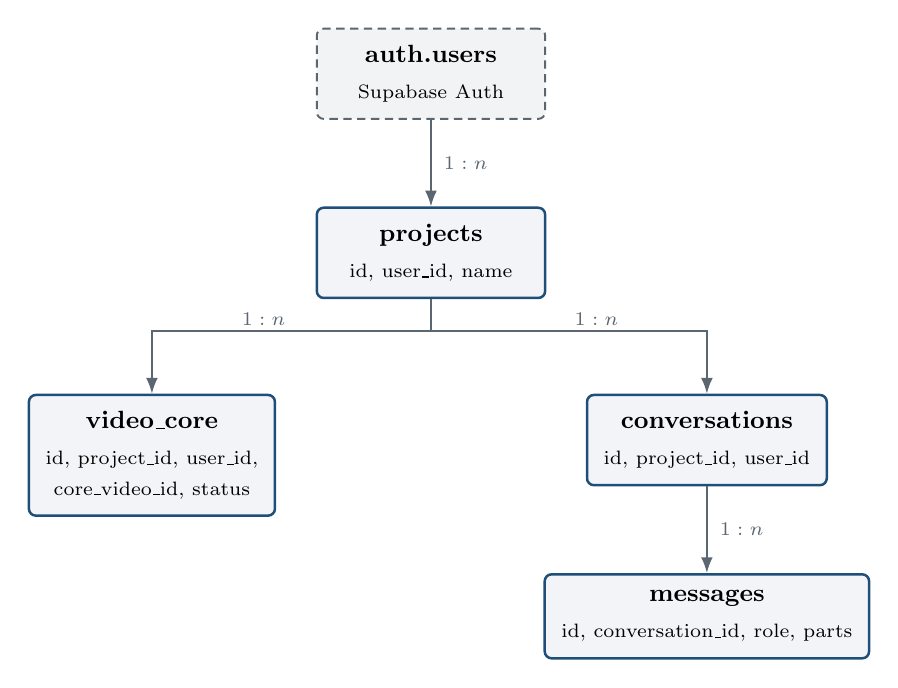
\begin{tikzpicture}

  \node[extbox] (users) {\textbf{auth.users}\\[2pt]\scriptsize Supabase Auth};
  \node[entity, below=11mm of users] (projects)
    {\textbf{projects}\\[2pt]\scriptsize id, user\_id, name};

  \node[entity, below left=12mm and 5mm of projects] (video)
    {\textbf{video\_core}\\[2pt]\scriptsize id, project\_id, user\_id,\\
     \scriptsize core\_video\_id, status};
  \node[entity, below right=12mm and 5mm of projects] (conv)
    {\textbf{conversations}\\[2pt]\scriptsize id, project\_id, user\_id};
  \node[entity, below=11mm of conv] (msg)
    {\textbf{messages}\\[2pt]\scriptsize id, conversation\_id, role, parts};

  \draw[rel] (users) -- node[card, right=1mm] {$1 : n$} (projects);
  \draw[rel] (projects.south) -- ++(0,-4mm) -| node[card, pos=0.3, above] {$1 : n$} (video.north);
  \draw[rel] (projects.south) -- ++(0,-4mm) -| node[card, pos=0.3, above] {$1 : n$} (conv.north);
  \draw[rel] (conv) -- node[card, right=1mm] {$1 : n$} (msg);

\end{tikzpicture}
\caption{Application database. Every relationship cascades on delete, so removing a
project removes its recordings, conversations and messages with it.}
\label{fig:erd}
\end{figure}

\subsubsection*{Physical schema}

\optfigure{falcon-vqa-schema.png}{Application database as deployed: the four live
relations with their columns, types and nullability, and their foreign keys into
\texttt{auth.users}. Filled markers denote non-nullable columns.}{0.92}{fig:schema}

\subsubsection*{\texttt{video\_core}}

This relation is the application's view of a recording analysed by the core service. It
is the only place where the two halves of the system meet, and three of its design
decisions are load-bearing.

\begin{table}[htbp]
\centering
\small
\begin{tabularx}{\textwidth}{@{}L{3.2cm}L{2.5cm}X@{}}
\toprule
\textbf{Column} & \textbf{Type} & \textbf{Purpose} \\
\midrule
\texttt{id} & \texttt{uuid} PK & Application identity, independent of the analysis service. \\
\texttt{project\_id} & \texttt{uuid} FK & Owning project; cascades on delete. \\
\texttt{user\_id} & \texttt{uuid} FK & Owning account; the column row-level security tests. \\
\texttt{title} & \texttt{text} & Display name, editable without affecting analysis. \\
\texttt{source\_type} & \texttt{text} & \texttt{upload} or \texttt{url}. \\
\texttt{storage\_path} & \texttt{text} & Object in the application project's bucket. \\
\texttt{source\_url} & \texttt{text} & The URL the analysis service was handed. \\
\texttt{core\_video\_id} & \texttt{text} & The content hash the analysis service identifies this recording by. Null until the bytes have been fetched. \\
\texttt{playback\_url} & \texttt{text} & The public MP4 in the analysis project's bucket; this is what actually plays. \\
\texttt{poster\_url} & \texttt{text} & Single frame written at ingest, for the workspace grid. \\
\texttt{duration}, \texttt{size\_bytes} & \texttt{numeric}, \texttt{bigint} & Reported back by the analysis service. \\
\texttt{status} & \texttt{text} & \texttt{pending}, \texttt{uploading}, \texttt{queued}, \texttt{analyzing}, \texttt{ready} or \texttt{failed}. \\
\texttt{job\_id} & \texttt{text} & The background job being polled. \\
\texttt{stage} & \texttt{text} & \texttt{fetching}, \texttt{chunking}, \texttt{analyzing}, \texttt{indexing}, \texttt{aggregating} or \texttt{complete}. \\
\texttt{progress} & \texttt{jsonb} & The job's last progress detail, rendered directly by the interface. \\
\texttt{error} & \texttt{text} & Failure reason, retained so the row explains itself. \\
\texttt{ingest\_config} & \texttt{jsonb} & What the pipeline was asked for: analyzers, mode, preset, weights, interval and duration bounds. \\
\texttt{analyzers} & \texttt{text[]} & What it actually produced. \\
\texttt{aggregates} & \texttt{text[]} & Which video-level results exist. \\
\texttt{chunk\_config} & \texttt{text} & The chunking scheme, e.g. \texttt{audio\_video:5-20}. \\
\texttt{chunk\_count} & \texttt{int} & Number of chunks produced. \\
\texttt{created\_at}, \texttt{updated\_at} & \texttt{timestamptz} & \texttt{updated\_at} is maintained by trigger. \\
\bottomrule
\end{tabularx}
\end{table}

\begin{enumerate}[label=\textbf{D-\arabic*.},leftmargin=3.0em]
  \item \textbf{Two URLs are kept, not one.} The system spans two Supabase projects: this
        one holds the row and the object the browser uploaded, while the analysis
        service's own project holds the canonical copy that plays.
        \texttt{source\_url} and \texttt{playback\_url} therefore point at different
        objects and both are retained.
  \item \textbf{Uniqueness is per project, never global.} Because
        \texttt{core\_video\_id} is the content hash, the same file added to two
        projects yields the same value. The unique index is declared over
        \texttt{(project\_id, core\_video\_id)} and is partial --- restricted to rows
        where the column is non-null, since the identifier does not exist until the
        bytes have been downloaded. Deleting one project's row must therefore not
        delete the analysis service's copy while another row still references it.
  \item \textbf{Produced analyzers are an array, not a document.} Both the interface and
        the agent evaluate \emph{``does this recording have people analysis?''} as a
        predicate, which an array answers directly and an opaque JSON document does not.
        The requested configuration, by contrast, is \texttt{jsonb}, because it is
        replayed verbatim on re-index rather than queried.
\end{enumerate}

\subsubsection*{Remaining relations}

\begin{table}[htbp]
\centering
\small
\begin{tabularx}{\textwidth}{@{}L{2.6cm}X@{}}
\toprule
\textbf{Relation} & \textbf{Columns and notes} \\
\midrule
\texttt{projects} & \texttt{id}, \texttt{user\_id}, \texttt{name}, \texttt{description}, timestamps. The grouping every other relation hangs from. \\
\texttt{conversations} & \texttt{id}, \texttt{user\_id}, \texttt{project\_id}, \texttt{title}, \texttt{lastContext}, timestamps. A conversation is optionally attached to a project; the attachment is what scopes the agent's tools. \\
\texttt{messages} & \texttt{id}, \texttt{conversation\_id}, \texttt{role}, \texttt{parts}, \texttt{metadata}, \texttt{created\_at}. \texttt{parts} is \texttt{jsonb} because a turn is a sequence of heterogeneous parts --- text, tool calls, tool results and artifacts --- whose shapes are set by the agent runtime. \\
\texttt{videos} & Superseded. The relation predates the current analysis service and is retained but no longer read by anything; \texttt{video\_core} replaced it additively so that no migration had to drop data. \\
\bottomrule
\end{tabularx}
\end{table}

\subsubsection*{Indexes, integrity and access control}

\begin{itemize}
  \item \textbf{Indexes.} \texttt{video\_core} is indexed on
        \texttt{(project\_id, created\_at DESC)} for the workspace listing, and partially
        on \texttt{job\_id} where it is non-null, which is the lookup that reconciliation
        performs. \texttt{conversations} is indexed on \texttt{project\_id} and
        \texttt{messages} on \texttt{(conversation\_id, created\_at)}, the order a
        conversation is replayed in.
  \item \textbf{Integrity.} Every foreign key cascades on delete, so a removed account or
        project leaves nothing orphaned. A shared trigger function maintains
        \texttt{updated\_at} on each relation that carries it.
  \item \textbf{Access control.} Row-level security is enabled on every relation.
        \texttt{projects}, \texttt{conversations} and \texttt{video\_core} test
        \texttt{auth.uid() = user\_id} directly. \texttt{messages} carries no owner
        column, so its policy tests ownership of the parent conversation through an
        \texttt{EXISTS} subquery --- the row is reachable only if the conversation it
        belongs to is. This is the database half of NFR-9; the other half is the
        project-scoping function through which the agent's tools resolve recording
        identifiers.
\end{itemize}

\subsection{Object Storage}

Two public buckets are used, one in each Supabase project.

\begin{table}[htbp]
\centering
\small
\begin{tabularx}{\textwidth}{@{}L{2.6cm}L{2.7cm}X@{}}
\toprule
\textbf{Bucket} & \textbf{Project} & \textbf{Contents and policy} \\
\midrule
\texttt{project-assets} & Application &
What the browser uploads, laid out per user and project. Public read; insert restricted
to authenticated accounts; delete restricted to the object's owner. \\
\texttt{videos} & Analysis service &
The canonical copy the pipeline reads, stored at
\texttt{\{video\_id\}/\{filename\}}, together with
\texttt{\{video\_id\}/poster.jpg}. Public read, so a playback URL is permanent and
unsigned. \\
\bottomrule
\end{tabularx}
\end{table}

Because the object path begins with the content hash, re-ingesting identical bytes
resolves to an object that already exists and the upload is skipped entirely. The
service checks for the object before writing rather than relying on overwrite semantics,
so a repeated ingest of a large recording costs nothing.

\subsection{Analysis Record Store}

One JSON document is written per recording, named
\texttt{\{sanitised-filename\}\_\_\{video\_id[:8]\}.json}. The filename carries a
human-readable stem so that a directory of records can be inspected directly, and the
truncated content hash so that two recordings sharing a name cannot collide. On
re-ingest, any existing document for the same identifier is removed before the new one
is written, so a stale record can never sit alongside a current one under a different
name.

\begin{table}[htbp]
\centering
\small
\begin{tabularx}{\textwidth}{@{}L{3.4cm}L{2.2cm}X@{}}
\toprule
\textbf{Field} & \textbf{Type} & \textbf{Contents} \\
\midrule
\texttt{video\_id} & string & Content hash; the identity every other store joins on. \\
\texttt{video\_url} & string & Public URL of the canonical copy. \\
\texttt{storage\_path} & string & Object path within the analysis bucket. \\
\texttt{source\_url} & string & Where the recording was fetched from. \\
\texttt{filename} & string & Original name, preserved for display. \\
\texttt{preset}, \texttt{params} & string, object & The chunking scheme and its duration bounds or weights. \\
\texttt{chunk\_config} & string & The composite key identifying that scheme. \\
\texttt{duration}, \texttt{size\_bytes} & number & Measured at ingest. \\
\texttt{poster\_url} & string & The extracted poster frame. \\
\texttt{analyzers} & array & Which analyzers ran. \\
\texttt{chunks} & array & One entry per chunk; see below. \\
\texttt{aggregates} & object & One key per aggregator, holding its full result. \\
\texttt{aggregates\_analyzers} & array & The analyzer set the aggregates were computed from, so a stale cache is detectable. \\
\bottomrule
\end{tabularx}
\end{table}

Each entry of \texttt{chunks} carries \texttt{id}, \texttt{start} and \texttt{end},
followed by \emph{one key per analyzer that produced output for that chunk}, whose value
is that analyzer's structured result --- \texttt{default\_video} holding the scene
schema, \texttt{people} holding per-person records with their box locations,
\texttt{ocr} holding the read texts, and so on. An analyzer that was gated out for a
chunk simply contributes no key, so absence is represented naturally rather than as a
null. This is precisely the shape a relational schema cannot accommodate without a
migration per analyzer.

Two conventions apply throughout. Keys prefixed with an underscore ---
\texttt{\_frames}, \texttt{\_detector\_labels} --- are provenance retained for debugging:
they record which frames a description was derived from and what the cheap detector
believed, and they are never embedded, never copied into a vector payload and never
returned by the API. And no local filesystem path is ever persisted; the cached file is
re-derived from \texttt{video\_id} on demand and re-downloaded if the cache is cold, so
a record remains correct after the data directory moves or the cache is wiped.

\subsection{Vector Store}

\subsubsection*{Collection and point structure}

A single Qdrant collection, \texttt{chunks}, holds one point per
\emph{(recording, analyzer, chunk span, chunk configuration)}. Each point carries all
five named vectors, each 384-dimensional and compared by cosine distance. Making the
point --- rather than the vector --- the unit of storage means a limit of ten returns ten
chunks, the payload is stored once, and a filter is evaluated once.

\begin{table}[htbp]
\centering
\small
\begin{tabularx}{\textwidth}{@{}L{2.5cm}X@{}}
\toprule
\textbf{Named vector} & \textbf{Embedded text} \\
\midrule
\texttt{combined}    & The whole flattened record. The default search space. \\
\texttt{description} & The prose description alone. \\
\texttt{people}      & Role, clothing and appearance, phrased as clauses. \\
\texttt{actions}     & What each subject did, or what each object was used for. \\
\texttt{objects}     & Object names, or the literal strings read from screen. \\
\bottomrule
\end{tabularx}
\end{table}

A vector space is omitted rather than written empty, so a chunk in which no person was
seen is not a candidate in a people-scoped search at all, instead of matching against
empty text.

\subsubsection*{Point identity}

The point identifier is a UUID derived deterministically from

\begin{center}
\texttt{sha1(video\_id | analyzer\_id | start | end | chunk\_config)}
\end{center}

so that re-ingesting the same chunk upserts in place rather than duplicating. The key is
built from the \emph{time span} rather than a positional index, because chunk 12 of one
chunking run is a different moment from chunk 12 of another and a positional identifier
would silently rebind a vector to the wrong timeframe. Custom chunking weights are
hashed into \texttt{chunk\_config} for the same reason: without it, two different
weightings sharing the same duration bounds would collide and the second ingest would
overwrite the first.

\subsubsection*{Payload and filters}

The payload carries everything required to rank, filter and cite a moment, so retrieval
never joins back to the record store: the recording identifier and playback URL, the
analyzer, chunk configuration and chunk identifier, the time span, the combined text and
description, the setting, the people, objects, actions and tags, the speakers and their
turns, the texts read from screen, the object detections, the full per-person records,
and the person count.

\begin{table}[htbp]
\centering
\small
\begin{tabularx}{\textwidth}{@{}L{2.5cm}L{2.4cm}L{1.9cm}X@{}}
\toprule
\textbf{Filter} & \textbf{Payload field} & \textbf{Match} & \textbf{Type} \\
\midrule
\texttt{video\_ids}    & \texttt{video\_id}     & any   & \texttt{list[str]} \\
\texttt{chunk\_ids}    & \texttt{chunk\_id}     & any   & \texttt{list[int]} \\
\texttt{analyzer\_ids} & \texttt{extractor\_id} & any   & \texttt{list[str]} \\
\texttt{chunk\_config} & \texttt{chunk\_config} & exact & \texttt{str} \\
\texttt{objects}       & \texttt{objects}       & any   & \texttt{list[str]} \\
\texttt{tags}          & \texttt{tags}          & any   & \texttt{list[str]} \\
\texttt{speakers}      & \texttt{speakers}      & any   & \texttt{list[str]} \\
\texttt{people}        & \texttt{people}        & any   & \texttt{list[str]} \\
\texttt{min\_people}   & \texttt{people\_count} & $\geq$ & \texttt{int} \\
\texttt{max\_people}   & \texttt{people\_count} & $\leq$ & \texttt{int} \\
\texttt{after}         & \texttt{start}         & $\geq$ & \texttt{float} \\
\texttt{before}        & \texttt{end}           & $\leq$ & \texttt{float} \\
\bottomrule
\end{tabularx}
\end{table}

The filter set is declared in one place and the API passes a flat dictionary through to
it, so a filter added to the declaration is reachable from the API immediately; the
previous hand-plumbed parameter list left six store filters silently unreachable. An
unrecognised filter name raises an error carrying the nearest valid name, because a
filter that is silently ignored returns plausible but wrong results, which is worse than
a failure.

The same twelve fields are declared as payload indexes. The person count is indexed
specifically because counting is what embeddings cannot do: a query for \emph{``mostly
empty store''} retrieved the busiest chunk in the recording, since a description listing
five people reads much the same to a vector as one listing two. In embedded mode Qdrant
ignores payload indexes and filtering scans instead --- correct, and acceptable at this
scale. The index declarations are retained so that pointing the same code at a Qdrant
server gains real indexes with no change.

Deletion is scoped rather than wholesale. Removing vectors takes an optional chunk
configuration and analyzer identifier, because re-running one analyzer must delete only
that analyzer's vectors; deleting by recording alone would destroy every other
analyzer's work, so adding one analyzer to an existing recording would silently discard
the rest.

\subsection{Cross-Store Identity}

The content hash is the single join key across all four stores. It is computed while the
bytes are being read, which is why the download must complete before the object's own
name exists.

\begin{figure}[htbp]
\centering
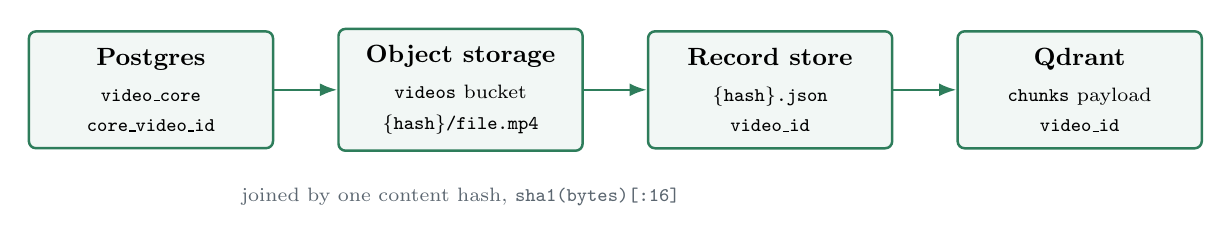
\begin{tikzpicture}

  \node[storebox] (pg)
    {\textbf{Postgres}\\[2pt]\scriptsize \texttt{video\_core}\\
     \scriptsize \texttt{core\_video\_id}};
  \node[storebox, right=8mm of pg] (obj)
    {\textbf{Object storage}\\[2pt]\scriptsize \texttt{videos} bucket\\
     \scriptsize \texttt{\{hash\}/file.mp4}};
  \node[storebox, right=8mm of obj] (rec)
    {\textbf{Record store}\\[2pt]\scriptsize \texttt{\{hash\}.json}\\
     \scriptsize \texttt{video\_id}};
  \node[storebox, right=8mm of rec] (qd)
    {\textbf{Qdrant}\\[2pt]\scriptsize \texttt{chunks} payload\\
     \scriptsize \texttt{video\_id}};

  \draw[keyflow] (pg) -- (obj);
  \draw[keyflow] (obj) -- (rec);
  \draw[keyflow] (rec) -- (qd);

  \node[card, below=4mm of obj.south] (note)
    {joined by one content hash, \texttt{sha1(bytes)[:16]}};

\end{tikzpicture}
\caption{The content hash of the video bytes is the identity shared by every store, which
is what makes ingestion idempotent (NFR-10).}
\label{fig:keys}
\end{figure}

Durability differs by store, and the difference is intentional:

\begin{itemize}
  \item The \textbf{record store} is authoritative. It holds the analyzer and aggregator
        output, which is the expensive artifact, and everything else can be rebuilt from
        it.
  \item The \textbf{vector store} is derived. Re-indexing rebuilds it from the records
        at the cost of local embedding alone, with no API spend and no re-analysis.
  \item The \textbf{media cache} is regenerable. Deleting it costs a re-download and
        never data, which is why no local path is persisted anywhere.
  \item \textbf{Job state} is deliberately in memory and does not survive a restart. The
        application detects the loss when a poll returns nothing, and either recovers
        the recording from its persisted record or fails the row explicitly so that
        re-indexing becomes the route forward.
\end{itemize}


\clearpage
\section{User Interface Design}

The interface is organised around a single principle: the operator should never be
required to scrub. Every screen terminates in a moment that plays.
Figure~\ref{fig:ui} shows the four principal states of the application: the project
workspace, the ingestion dialog, the agent chat with its clip reel and timeline studio,
and the per-recording detail view.

\optfigure{falcon-vqa-ui-design.png}{Operator interface. Clockwise from top left: the
project workspace and video grid; the ingestion dialog, whose analyzer list is built
from the analysis service's own capability endpoint; the per-recording detail view with
its chunk map and tabbed record; and the agent chat with the clip reel artifact panel
and the timeline studio.}{1.0}{fig:ui}

\begin{table}[htbp]
\centering
\small
\begin{tabularx}{\textwidth}{@{}L{3.4cm}X@{}}
\toprule
\textbf{Screen} & \textbf{Operator activity} \\
\midrule
Landing and documentation & Presents the system and hosts the full documentation: concepts, workspace guides, and the API reference. \\
Authentication  & Registration and sign-in. Every subsequent route is guarded, and every query is restricted to the signed-in account. \\
Projects        & Lists projects, each grouping a set of recordings. Opening one enters its workspace. \\
Workspace       & Adds recordings by file or by link, selects the analyzers and the chunking mode, and observes each recording advance through Uploading, Indexing and Ready. Only ready recordings may be searched, and the interface states this rather than returning an empty result. \\
Agent chat      & Accepts a description or a question, and a selection of recordings to consider. The assistant chooses the retrieval operations, and answers remain concise and cite timecodes. Conversations persist and may be resumed. \\
Clip reel panel & Opens beside the chat whenever the results are moments. A player is placed above the list of moments; selecting one plays it, and they may be played consecutively as a reel. \\
Timeline studio & Presents the recording's scenes, transcript and chapters against a timeline that follows the playhead, for reviewing what was indexed in the region being watched. \\
Recording detail & Five tabs over one recording: Overview for the video-level output, Chunks for the chunk map and per-chunk records, Speech for the transcript, People and objects for linked entities and their timelines, and Record for the raw stored document. \\
\bottomrule
\end{tabularx}
\end{table}

Three decisions in the interface follow directly from the requirements. Progress is
reported per recording rather than as a global spinner, so that a workspace with several
recordings being processed at once remains legible (FR-3). A recording that is not yet
ready is excluded from search with a stated reason instead of silently returning nothing,
because an empty result and an unfinished index are different situations that look
identical to the operator. And every result carries its timecode as the primary handle,
since the timecode is what turns a search result into footage the operator can watch.


\clearpage
\section{Acceptance Test Cases and Test Plan}

This section states what has to be true for the system to be accepted, gives the test
cases that establish it, and then sets out the plan under which those cases are run:
the environment, the test data, the entry and exit criteria, what is automated, and how
failures are recorded.

\subsection{Acceptance Criteria}

Every requirement from Section~3 is restated below as a condition that can be observed
to hold or not hold, together with the cases that establish it. A requirement with no
case would be a requirement nobody agreed how to check, so the third column is also the
traceability matrix.

\begin{table}[htbp]
\centering
\footnotesize
\begin{tabularx}{\textwidth}{@{}L{1.2cm}XL{2.7cm}@{}}
\toprule
\textbf{Req.} & \textbf{Accepted when} & \textbf{Verified by} \\
\midrule
FR-1  & An operator can register, sign in and group recordings into projects, and no account can reach another account's projects, recordings or conversations by any route. & AT-01 to AT-04, AT-06 \\
FR-2  & A recording can be added by file or by link, the selected analyzers are the ones that run, and the recording reaches \texttt{ready}. & AT-07, AT-08, AT-09 \\
FR-3  & Stage and progress are visible throughout processing, the rest of the workspace stays usable, and a failure explains itself instead of hanging. & AT-11, AT-12, AT-17, AT-18 \\
FR-4  & A described event is returned within the leading results, and content that is absent is reported as absent. & AT-19, AT-20, AT-24 \\
FR-5  & Restricting by time, by content or by recording removes non-matching results and retains matching ones. & AT-21, AT-22, AT-23 \\
FR-6  & An answer is correct against the ground-truth sheet, carries a timecode for every claim, and is refused when the footage does not support it. & AT-27, AT-28, AT-29 \\
FR-7  & Selecting a result plays the footage from that moment with no scrubbing, individually or as a reel. & AT-32, AT-33 \\
FR-8  & Summary, chapters, events, entities and anomalies are produced for a recording and are legible without watching it. & AT-35, AT-37, AT-38 \\
FR-9  & A multi-turn conversation selects the right tools without the recording being named each turn, and survives being reopened. & AT-30, AT-31 \\
FR-10 & The stored record for any chunk is retrievable, and the timeline follows the playhead. & AT-34, AT-36 \\
FR-11 & A recording can be re-examined at another depth without being re-added, and earlier results survive. & AT-14, AT-15 \\
FR-12 & Every retrieval capability is reachable over the documented API, and a client can be built from the capability endpoint alone. & AT-26, AT-39, AT-41 \\
\midrule
NFR-1  & Search returns within 2\,s and an answer within 15\,s on a warm instance. & PT-1, PT-2 \\
NFR-2  & A recording becomes searchable within roughly three times its own duration. & PT-3 \\
NFR-3  & Stage and progress refresh at least every 5\,s during ingestion. & AT-11, PT-4 \\
NFR-4  & Playback of a selected moment begins within 2\,s, including the second and later moments of a reel. & AT-32, AT-33, PT-5 \\
NFR-5  & No answer is produced without citations, and an unsupported question is declined. & AT-27, AT-29 \\
NFR-6  & Silent, cut-free, fixed-camera footage yields multiple usable chunks rather than one span. & AT-16 \\
NFR-7  & Deselecting an analyzer avoids its cost, a gated frame incurs no model call, and reviewing existing results incurs none. & AT-09, AT-26, AT-38, PT-3, PT-6 \\
NFR-8  & A new analyzer appears in the API and the ingest dialog after one module and one registry line, with no other edit. & AT-10, AT-40 \\
NFR-9  & Isolation holds at the database and at the agent boundary, including against a fabricated identifier. & AT-03 to AT-06 \\
NFR-10 & The same file submitted twice is recognised as one recording and is neither stored nor processed twice. & AT-13 \\
\bottomrule
\end{tabularx}
\end{table}

\subsection{Case Format and Severity}

Each case below gives its precondition, the procedure to follow, and the result that
constitutes a pass. Cases are grouped by the area they exercise and are intended to be
run in order within a group, since later cases in a group often depend on state the
earlier ones create. The fixtures named in the procedures are specified in
Section~9.11, and the pass conditions for search and question cases are scored against
the ground-truth sheets described there rather than against a tester's impression at
the time.

Severity is assigned to a failure as follows. \textbf{Critical} means the system cannot
be used for its purpose, or a tenant can reach another tenant's data. \textbf{Major}
means a stated requirement is not met but a workaround exists. \textbf{Minor} means the
result is correct but the presentation or the timing is not what was intended.

\subsection{Test Cases: Accounts and Tenancy}

\begin{table}[htbp]
\centering
\footnotesize
\begin{tabularx}{\textwidth}{@{}L{0.9cm}L{3.2cm}XX@{}}
\toprule
\textbf{ID} & \textbf{Case and precondition} & \textbf{Procedure} & \textbf{Expected result} \\
\midrule

AT-01 & Registration and sign-in. No account exists for the address used. &
1) Register with an address and password. 2) Sign out. 3) Sign in again. 4) Request a
guarded route while signed out. &
The account is created and the session is established. Step 4 redirects to sign-in
rather than rendering the route or returning data. \\

AT-02 & Project creation and listing. Account A signed in. &
1) Create two projects. 2) Return to the project list. 3) Open one. 4) Rename it. &
Both projects appear, newest first. Opening one enters its workspace. The rename is
reflected in the list without a reload. \\

AT-03 & Cross-account isolation. Account A owns a project holding a ready recording and
a saved conversation. &
1) Sign in as B. 2) Inspect the project list, the workspace and the conversation list. &
B sees none of A's projects, recordings, conversations or messages. B's own lists are
empty rather than populated with A's rows. \\

AT-04 & Access by identifier. A's project, recording and conversation identifiers are
known. Signed in as B. &
1) Request each of A's identifiers directly by URL. 2) Repeat against the client's own
API routes. &
Every request is refused or returns empty. No row belonging to A is returned by any
route, which is row-level security rather than interface filtering. \\

AT-05 & Agent scoping against a fabricated identifier. B signed in, conversation
attached to B's project. &
1) Ask the agent a question naming a recording identifier that belongs to A. &
The identifier is filtered out by the project scoping function. The agent answers from
B's own recordings or states that the recording is not in this project. It never
returns content from A's footage. \\

AT-06 & Cascading delete. A owns a project with recordings, a conversation and messages. &
1) Delete the project. 2) Query for the child rows directly. &
Recordings, conversations and messages belonging to the project are gone. No orphaned
row remains. \\

\bottomrule
\end{tabularx}
\end{table}

\subsection{Test Cases: Ingestion and Processing}

\begin{table}[htbp]
\centering
\footnotesize
\begin{tabularx}{\textwidth}{@{}L{0.9cm}L{3.2cm}XX@{}}
\toprule
\textbf{ID} & \textbf{Case and precondition} & \textbf{Procedure} & \textbf{Expected result} \\
\midrule

AT-07 & Add a recording by upload. Empty project. &
1) Open the ingest dialog. 2) Select \texttt{cctv-shopping}. 3) Accept the default
analyzers and chunking mode. 4) Submit and wait. &
The recording appears immediately with a poster frame, advances through its stages, and
reaches \texttt{ready}. Chunk count and duration are populated. \\

AT-08 & Add a recording by link. A reachable direct video URL. &
1) Choose the link tab. 2) Paste the URL. 3) Submit and wait. &
The service fetches the file, hashes it, and the recording reaches \texttt{ready} with
the same behaviour as an upload. \texttt{source\_url} and \texttt{playback\_url} both
resolve. \\

AT-09 & Analyzer selection is honoured. Ingest dialog open. &
1) Deselect people and text recognition, leaving scene and transcription. 2) Ingest. 3)
Inspect the stored record and the recording's analyzer list once ready. &
Only the selected analyzers appear in the produced list. No chunk carries a key for a
deselected analyzer, and no cost was incurred for one. \\

AT-10 & Analyzer list is discovered, not hard-coded. Analysis service running. &
1) Open the ingest dialog. 2) Compare its analyzer list against the capability
endpoint's response. &
The two agree exactly. The dialog builds its list from the endpoint rather than from a
list compiled into the client. \\

AT-11 & Progress is visible and the interface stays usable. Ingestion of a 5-minute
recording in progress. &
1) Observe the recording card throughout. 2) While it processes, open another recording
and run a search. &
Stage and progress update at least every 5 seconds and move monotonically through
fetching, chunking, analyzing, indexing and aggregating. The rest of the workspace
remains responsive. \\

AT-12 & Only ready recordings are searchable. A recording mid-ingest. &
1) Attempt to include it in a search or a question. &
The interface states that the recording is still being processed. It does not return an
empty result set that would read as nothing found. \\

AT-13 & Idempotent ingestion. \texttt{cctv-shopping} already ingested into project P. &
1) Add the identical file again to project P. 2) Add it to a second project Q. 3)
Inspect the object storage path and the record store. &
In P the file is recognised as the same recording by its content hash: it is not
uploaded, re-analysed or duplicated. In Q a separate row exists, but both rows share one
\texttt{core\_video\_id}, one stored object and one record document. \\

AT-14 & Re-examine at a different depth. A recording indexed at
\texttt{audio\_video:5-20}. &
1) Re-index with a different chunking configuration. 2) Search against each
configuration in turn. &
Both chunkings coexist. Vectors from the first are not overwritten, and a search scoped
to one configuration returns only that configuration's chunks. \\

AT-15 & Adding one analyzer to an existing recording. A recording indexed without text
recognition. &
1) Re-run with text recognition added. 2) Inspect the other analyzers' chunk records and
vectors. &
Text recognition output appears. Every previously produced analyzer's records and
vectors are intact, because deletion is scoped to the analyzer being re-run. \\

AT-16 & Silent, cut-free footage. \texttt{cctv-shopping}, which has neither speech nor
hard cuts. &
1) Ingest with the default preset. 2) Inspect the resulting chunk boundaries and
descriptions. &
Multiple chunks are produced, not one span covering the whole recording. Weight
redistribution puts the load on the signals that fired. Descriptions differ between
chunks. \\

AT-17 & Failed ingestion explains itself. A URL that does not resolve to a video. &
1) Submit it. 2) Observe the recording card. &
The recording reaches \texttt{failed}, the reason is retained on the row and shown, and
the failure does not leave the workspace in a loading state. \\

AT-18 & Lost job recovery. Ingestion in progress. &
1) Restart the analysis service mid-ingest. 2) Let the client poll. &
The client detects that the job no longer exists and either recovers the recording from
its persisted record or fails the row explicitly, so that re-indexing is available.
It does not poll indefinitely. \\

\bottomrule
\end{tabularx}
\end{table}

\subsection{Test Cases: Search and Filtering}

\begin{table}[htbp]
\centering
\footnotesize
\begin{tabularx}{\textwidth}{@{}L{0.9cm}L{3.2cm}XX@{}}
\toprule
\textbf{ID} & \textbf{Case and precondition} & \textbf{Procedure} & \textbf{Expected result} \\
\midrule

AT-19 & Search by description. \texttt{cctv-shopping} ready, ground-truth sheet written. &
1) Take five events from the sheet. 2) Search for each in natural language, using
wording that does not repeat the stored description. 3) Record the rank of the correct
moment. &
For each query the correct moment is within the top three results, and its timecode is
within one chunk of the ground-truth timecode. \\

AT-20 & Vector space scoping. Same fixture. &
1) Search for a person by clothing, scoped to the people vector space. 2) Repeat against
the combined space. &
The people-scoped search ranks the correct person higher, because the query is matched
against a short person description rather than the whole chunk record. \\

AT-21 & Time filter. Same fixture. &
1) Search for an event known to occur late in the recording. 2) Repeat restricted to the
first 60 seconds. &
The unrestricted search returns the moment. The restricted search excludes it, and every
returned span lies inside the requested window. \\

AT-22 & Content filters. Same fixture. &
1) Filter by an object known to appear. 2) Filter by a minimum person count of three. 3)
Filter by a speaker on the multi-speaker fixture. &
Each filter removes non-matching chunks and retains matching ones. The person count
filter answers a counting query that description similarity alone gets wrong. \\

AT-23 & Recording scope. Two ready recordings in one project. &
1) Search with both selected. 2) Search with one selected. &
The scoped search returns results only from the selected recording. \\

AT-24 & Absent content is reported as absent. Any ready recording. &
1) Search for something the ground-truth sheet confirms is not present. &
The score threshold suppresses the nearest neighbours and the result is empty, rather
than the top-ranked unrelated chunk being presented as a match. \\

AT-25 & Unknown filter is rejected. Direct API access. &
1) Issue a search carrying a misspelled filter name. &
The request fails with an error naming the nearest valid filter. The filter is not
silently ignored, which would return plausible but wrong results. \\

AT-26 & Response detail levels. Direct API access. &
1) Issue the same search at \texttt{minimal}, \texttt{standard} and \texttt{full}. 2)
Compare the payloads. &
All three return the same ranked moments. The payload grows with the level, and
\texttt{minimal} is small enough to be economical for an agent. \\

\bottomrule
\end{tabularx}
\end{table}

\subsection{Test Cases: Question Answering and Conversation}

\begin{table}[htbp]
\centering
\footnotesize
\begin{tabularx}{\textwidth}{@{}L{0.9cm}L{3.2cm}XX@{}}
\toprule
\textbf{ID} & \textbf{Case and precondition} & \textbf{Procedure} & \textbf{Expected result} \\
\midrule

AT-27 & Answer with citations. \texttt{cctv-shopping} ready. &
1) Ask five questions drawn from the ground-truth sheet. 2) Check each claim against the
sheet. 3) Follow each citation. &
Every answer is factually correct against the sheet. Every claim carries a timecode
reference, and following a reference plays footage that supports the claim. \\

AT-28 & Routing to the right aggregate. Same fixture, aggregates computed. &
1) Ask about a specific person. 2) Ask what was unusual. 3) Ask how busy the store was.
4) Inspect the routing recorded on each response. &
The person question routes to entities, the unusual question to novelty, the busyness
question to statistics. Routing is reported so that the answer can be traced. \\

AT-29 & Unanswerable question. Any ready recording. &
1) Ask about something the footage does not show, phrased as though it does. &
The system states that the footage does not support an answer. It does not synthesise a
plausible answer, and it does not cite an unrelated moment as evidence. \\

AT-30 & Multi-turn conversation. Project with two ready recordings. &
1) Ask an opening question. 2) Ask three follow-ups that refer back by pronoun without
naming the recording. 3) Observe the tools the agent selects. &
Context carries across turns. The agent chooses search, question or inspection
operations appropriately without the recording being named again. \\

AT-31 & Conversation persistence. A conversation with several turns. &
1) Leave the page. 2) Sign out and back in. 3) Reopen the conversation. &
Every turn is restored in order, including tool calls, results and artifacts. Continuing
the conversation retains the earlier context. \\

\bottomrule
\end{tabularx}
\end{table}

\subsection{Test Cases: Review, Playback and Inspection}

\begin{table}[htbp]
\centering
\footnotesize
\begin{tabularx}{\textwidth}{@{}L{0.9cm}L{3.2cm}XX@{}}
\toprule
\textbf{ID} & \textbf{Case and precondition} & \textbf{Procedure} & \textbf{Expected result} \\
\midrule

AT-32 & Play a result at its moment. A search returning several moments. &
1) Select a result. 2) Observe where playback begins. &
Playback starts at the result's start timecode with no manual scrubbing, and stops at
its end. \\

AT-33 & Clip reel. Several results drawn from one recording. &
1) Open the clip reel panel. 2) Play the moments consecutively. &
The moments play one after another. The MP4 is loaded once and seeked, so the second
and later moments start without a fresh load. \\

AT-34 & Timeline studio. A ready recording open. &
1) Play the recording. 2) Watch the scene, transcript and chapter tracks. 3) Scrub to a
new position. &
The timeline follows the playhead, and the region shown corresponds to what was indexed
at that position. Scrubbing moves the tracks with it. \\

AT-35 & Video-level review. \texttt{cctv-shopping} ready with aggregates computed. &
1) Open the recording detail view. 2) Read the summary, chapters, events, entities and
anomalies without watching the footage. 3) Compare against the ground-truth sheet. &
Each aggregate is produced and legible. The summary and chapters describe what actually
occurs. Anomalies flag moments the sheet marks as unusual. \\

AT-36 & Index inspection. Same fixture. &
1) Open the chunk map. 2) Select a chunk. 3) Read its stored record across the tabs. &
The description, on-screen text, people, objects and speech recorded for that chunk are
all retrievable, including the raw stored document. \\

AT-37 & Entity linking within a recording. A fixture in which one person appears
several times. &
1) Open the people and objects tab. 2) Follow one person's timeline. &
Separate sightings of the same person are linked into one individual with an ordered
account of what they did. Two people visible in the same chunk are never merged. \\

AT-38 & Aggregate caching. Aggregates already computed. &
1) Reopen the detail view. 2) Re-request the aggregates. &
Cached results are returned with no re-analysis and no model spend. Changing the
analyzer set marks the cache stale and triggers recomputation. \\

\bottomrule
\end{tabularx}
\end{table}

\subsection{Test Cases: Programmatic Access}

\begin{table}[htbp]
\centering
\footnotesize
\begin{tabularx}{\textwidth}{@{}L{0.9cm}L{3.2cm}XX@{}}
\toprule
\textbf{ID} & \textbf{Case and precondition} & \textbf{Procedure} & \textbf{Expected result} \\
\midrule

AT-39 & Client built from the capability endpoint alone. A ready recording; no access to
the source. &
1) Request the capability endpoint. 2) Using only its response, construct and issue a
valid search with a filter. &
The endpoint describes every analyzer, vector field, filter and aggregator needed. The
constructed request succeeds. \\

AT-40 & A new analyzer requires no client change. Analysis service source available. &
1) Register a trivial analyzer as one module and one registry line. 2) Restart the
service. 3) Reload the ingest dialog and the capability endpoint. &
The analyzer appears in both without any edit to ingestion, storage, the API or the
client. \\

AT-41 & Documented API matches behaviour. Documentation site deployed. &
1) Take each endpoint from the API reference. 2) Issue it against the running service. &
Every documented endpoint exists, accepts the documented parameters and returns the
documented shape. \\

\bottomrule
\end{tabularx}
\end{table}

\subsection{Non-Functional Verification}

The requirements that state a figure are verified by measurement rather than by
observation. Each is measured on a warm instance, repeated ten times, and reported as
the median together with the slowest of the ten, because a target met on average but
missed regularly is not met.

\begin{table}[htbp]
\centering
\small
\begin{tabularx}{\textwidth}{@{}L{1.1cm}L{3.0cm}XL{1.6cm}@{}}
\toprule
\textbf{ID} & \textbf{Measurement} & \textbf{Method} & \textbf{Target} \\
\midrule
PT-1 & Search latency &
Time from request to ranked moments at the API, and to rendered results in the browser,
over ten distinct queries against a 5-minute recording. & $\leq 2$\,s (NFR-1) \\
PT-2 & Answer latency &
Same method, over ten questions spanning the routed aggregates. & $\leq 15$\,s (NFR-1) \\
PT-3 & Processing time &
Wall-clock from submission to \texttt{ready}, divided by the recording's own duration,
with the default analyzer set. & $\leq 3\times$ duration (NFR-2) \\
PT-4 & Progress refresh &
Interval between successive stage or progress updates observed on the recording card
during a full ingest. & $\leq 5$\,s (NFR-3) \\
PT-5 & Playback latency &
Time from selecting a result to the first frame at that timecode, for a first moment and
for a subsequent moment in the same reel. & $\leq 2$\,s (NFR-4) \\
PT-6 & Response size &
Token count of an identical five-hit search at each detail level, so that the cost of the
agent path is known rather than assumed. & Recorded \\
\bottomrule
\end{tabularx}
\end{table}

Cost control (NFR-7) is verified alongside PT-3 by counting model calls: a re-run of an
aggregator over stored records must issue no analyzer calls, and a gated frame must issue
none at all. Robustness (NFR-6) is not a figure and is covered by AT-16.

\subsection{Test Environment}

The cases above are run against a deployed instance over HTTP and through the browser,
not against modules in isolation, because several of the defects found during
development (stale background jobs, broken answer synthesis, media paths that resolved
locally but not remotely) were only visible once the whole system was running.
Unit-level behaviour of individual analyzers and detectors is out of scope here.

\begin{table}[htbp]
\centering
\small
\begin{tabularx}{\textwidth}{@{}L{3.4cm}X@{}}
\toprule
\textbf{Element} & \textbf{Configuration under test} \\
\midrule
Analysis service & Python 3.13 and FastAPI on a CUDA-capable host, RTX 4060 with 8\,GB
VRAM, 16\,GB system RAM. Served over HTTP with Uvicorn, not with the reload server. \\
Client & Next.js production build, deployed on Vercel, pointed at the analysis service
by environment variable. \\
Application data & A dedicated Supabase project with row-level security enabled and the
schema migrations applied from a clean state. \\
Vector store & Qdrant in embedded mode, backed by a data directory that is emptied
before a full test pass. \\
Browsers & Chrome and Firefox, current stable releases, on a desktop viewport. \\
Accounts & Two registered accounts, A and B, used for every isolation test. Neither is
an administrator. \\
Model providers & Live API keys for the vision and language models, and a Hugging Face
token for the gated diarization model. Tests are not run against mocked providers,
because provider behaviour is part of what is being accepted. \\
\bottomrule
\end{tabularx}
\end{table}

Latency cases are run warm, meaning model weights are already resident and the media
cache holds the recording. Cold-start timings are recorded separately and reported as
such rather than being counted against the response targets, since a first request pays
for model loading that no subsequent request repeats.

\subsection{Test Data}

The same six recordings are used throughout, so that a result observed in one case can be
compared against the same footage in another. Each fixture was chosen because it isolates
a property the others do not exercise.

\begin{table}[htbp]
\centering
\small
\begin{tabularx}{\textwidth}{@{}L{3.0cm}L{3.4cm}X@{}}
\toprule
\textbf{Fixture} & \textbf{Content} & \textbf{Property it isolates} \\
\midrule
\texttt{cctv-shopping} & 5 minutes, 1280$\times$720, fixed camera, no speech &
The principal fixture. Neither cuts nor audio, which is the case general-purpose tools
fail on. Used for chunking, scene, people, object and text cases. \\
\texttt{chernobyl-\allowbreak audio-video} & 60 seconds, several speakers &
The only fixture in which speaker change, silence and speaker-attributed transcription
all fire. Used for every audio path. \\
\texttt{cctv-license-plate} & Short fixed-camera clip, vehicle plates &
On-screen text recognition against low-contrast, small-format text. \\
\texttt{cctv-fire}, \texttt{cctv-car-fire} & Short fixed-camera clips &
Novelty detection and event extraction, where the anomalous moment is known in advance. \\
\texttt{cctv-suspect} & Short fixed-camera clip, suspected theft &
Person description and the moments used in clip reel testing. \\
Extended set (planned) & Longer footage, multiple cameras, one shared subject &
Required for cross-recording person linking, which cannot be tested on footage that
shares no people. Recorded as a known gap in Section~6. \\
\bottomrule
\end{tabularx}
\end{table}

For each fixture, a ground-truth sheet is written before testing begins: a list of what
occurs in the recording and the timecode at which it occurs. Search and question cases
are scored against that sheet, so that a re-run of the same case on a later build is
comparable.

\subsection{Entry, Exit and Suspension}

\begin{table}[htbp]
\centering
\small
\begin{tabularx}{\textwidth}{@{}L{2.8cm}X@{}}
\toprule
\textbf{Criterion} & \textbf{Condition} \\
\midrule
Entry & The full pipeline runs end to end on at least one fixture; the client is
deployed and reaches the analysis service; migrations are applied; both test accounts
exist; ground-truth sheets are written. \\
Exit & Every Critical and Major case passes. No Critical or Major defect is open. Any
open Minor defect is recorded with the reason it is accepted. Every requirement in
Section~9.1 traces to at least one passing case. \\
Suspension & Testing stops if the analysis service is unreachable, a model provider is
returning errors, or a defect prevents ingestion from completing, since almost every
later case depends on an indexed recording. \\
Resumption & Testing resumes from the start of the group in which it was suspended,
not from the individual case, because a suspended run may have left partial state. \\
\bottomrule
\end{tabularx}
\end{table}

\subsection{Test Automation}

Not every case is worth automating. The ones that are worth automating are those run
repeatedly whose pass condition a machine can check: an HTTP status, a rank, a count, a
returned identifier. The ones that are not are those whose pass condition is a judgement
about footage, and those stay manual. The split is set out below.

\begin{table}[htbp]
\centering
\small
\begin{tabularx}{\textwidth}{@{}L{2.9cm}L{3.0cm}X@{}}
\toprule
\textbf{Layer} & \textbf{Tooling} & \textbf{What it covers} \\
\midrule
API regression &
Postman collection with an environment file, run headless by Newman &
Every endpoint in the API reference, with assertions on status, response shape and the
capability endpoint's contents. Covers AT-25, AT-26, AT-39 and AT-41 directly, and
builds on the collection already maintained alongside the service documentation. \\
Retrieval scoring &
A Python harness over the ground-truth sheets &
Issues the recorded queries against a live server and asserts the rank of the expected
moment and the timecode it resolves to. This is what turns AT-19 to AT-24 from a
subjective judgement into a number comparable across builds. \\
Pipeline benchmarks &
The existing \texttt{scripts/bench.py} &
Per-stage timings for detectors, fusion, chunking and export on a fixture, which is the
instrument PT-3 reads. Extended to record search and answer latency for PT-1 and PT-2. \\
Tenancy checks &
SQL assertions run as each test account &
Attempts a read of the other account's rows in every table and asserts that nothing is
returned. Covers AT-03, AT-04 and AT-06, which are the cases most costly to get wrong
and least interesting to repeat by hand. \\
Browser flows &
Playwright &
Sign-in, project creation, ingest to \texttt{ready}, search, and playback starting at the
expected timecode. Covers the happy path of AT-01, AT-02, AT-07, AT-11 and AT-32. \\
\midrule
Manual only &
Structured checklist against the ground-truth sheets &
Whether a description is a fair account of the footage, whether a summary reads
sensibly, whether linked people are the same person, and whether an answer is genuinely
supported by the moment it cites. These are AT-27, AT-28, AT-35 and AT-37, and a machine
scoring them would only be checking one model against another. \\
\bottomrule
\end{tabularx}
\end{table}

Two constraints shape how far automation is taken. The pipeline needs a GPU and live
model providers, so the suite cannot run on a hosted runner without one, and a full
ingest of the principal fixture costs real money on every run. The suite is therefore
split: the API regression, tenancy checks and browser flows run against a pre-indexed
fixture and are cheap enough to run on every change, while the retrieval scoring and
benchmark runs, which require a fresh ingest, are run before a release rather than on
every commit.

\subsection{Defect Recording and Reporting}

Each executed case is recorded with its identifier, the build and fixture it ran against,
the observed result, and a pass or fail verdict. A failure is logged with its severity,
the request or interaction that produced it, and whatever the system reported at the
time. Because ingestion runs as a background job, a failure during processing is recorded
together with the stage the job had reached and the reason retained on the recording row,
since that is usually the only account of what went wrong.

A defect is closed when the case that found it passes on a later build and the cases
around it in the same group still pass. A fix that repairs one case and breaks its
neighbour is not a fix, which is why the resumption rule above restarts a group rather
than a single case.


\clearpage
\section{Execution Plan}

\subsection{Schedule}

Development proceeds in eight phases. Each phase is validated end to end before the
next is begun, so that a defect in an earlier stage is not discovered through the
behaviour of a later one.

\begin{table}[htbp]
\centering
\small
\begin{tabularx}{\textwidth}{@{}L{1.9cm}L{4.0cm}X@{}}
\toprule
\textbf{Phase} & \textbf{Stage} & \textbf{Work} \\
\midrule
Phase 1 & Chunking &
Boundary detectors, weighted fusion, the three chunking modes and the duration bounds.
Validated on cut-free footage before anything was built upon it. \\
Phase 2 & Analysis &
Scene, people, object, text and speech analyzers; frame sampling; detector gating; and
the registry that renders them interchangeable. \\
Phase 3 & Indexing and retrieval &
Local embedding, the five named vectors, the typed filter set, response detail levels
and the search endpoint. \\
Phase 4 & Aggregation &
Video-level output, dependency ordering, caching, and person and object entity
linking. \\
Phase 5 & Question answering &
Routing of questions to the aggregates capable of answering them, and answer synthesis
with mandatory citations. \\
Phase 6 & Application tier &
Authentication and row-level security, projects and workspace, upload and status
reconciliation, the agent tool layer, clip reel and timeline studio, and the
per-recording detail view. \\
Phase 7 & Documentation &
The MDX documentation site --- concepts, workspace guides and the complete API
reference --- and the public landing pages. \\
Phase 8 & Hardening and reporting &
Acceptance tests against a live server, error handling, deployment, and this document.
\\
\bottomrule
\end{tabularx}
\end{table}

\subsection{Distribution of Work}

The project is undertaken by two members. The division follows the pipeline:
everything from a recording arriving to its being chunked and stored on one side, and
everything from a chunk being analysed to a question being answered on the other.

\begin{table}[htbp]
\centering
\small
\begin{tabularx}{\textwidth}{@{}L{4.2cm}X@{}}
\toprule
\textbf{Member} & \textbf{Responsibility} \\
\midrule
Avinash Anish &
\textbf{Application tier and ingestion.} The entire interface --- authentication,
projects and workspace, upload and status, agent chat, clip reel panel, timeline studio
and the recording detail view --- together with the agent tool layer and its project
scoping. On the pipeline side, ingestion: source handling, object storage and caching,
content-addressed identity, the four boundary detectors, weighted fusion and the three
chunking modes, and the background job and progress reporting behind them. \\
Vaivaswat Verma &
\textbf{Analysis service and retrieval.} Everything downstream of chunking: the
analyzers with their frame sampling and detector gating, embedding and the vector
store, filters and detail levels, the video-level aggregators including person and
object entity linking, and question routing and answer synthesis. Owns the HTTP API
through which these are exposed. \\
\midrule
Shared &
Architecture and design decisions, acceptance testing against a live server,
deployment, and documentation. \\
\bottomrule
\end{tabularx}
\end{table}


\end{document}
